% Options for packages loaded elsewhere
\PassOptionsToPackage{unicode}{hyperref}
\PassOptionsToPackage{hyphens}{url}
%
\documentclass[
]{book}
\usepackage{amsmath,amssymb}
\usepackage{lmodern}
\usepackage{iftex}
\ifPDFTeX
  \usepackage[T1]{fontenc}
  \usepackage[utf8]{inputenc}
  \usepackage{textcomp} % provide euro and other symbols
\else % if luatex or xetex
  \usepackage{unicode-math}
  \defaultfontfeatures{Scale=MatchLowercase}
  \defaultfontfeatures[\rmfamily]{Ligatures=TeX,Scale=1}
\fi
% Use upquote if available, for straight quotes in verbatim environments
\IfFileExists{upquote.sty}{\usepackage{upquote}}{}
\IfFileExists{microtype.sty}{% use microtype if available
  \usepackage[]{microtype}
  \UseMicrotypeSet[protrusion]{basicmath} % disable protrusion for tt fonts
}{}
\makeatletter
\@ifundefined{KOMAClassName}{% if non-KOMA class
  \IfFileExists{parskip.sty}{%
    \usepackage{parskip}
  }{% else
    \setlength{\parindent}{0pt}
    \setlength{\parskip}{6pt plus 2pt minus 1pt}}
}{% if KOMA class
  \KOMAoptions{parskip=half}}
\makeatother
\usepackage{xcolor}
\usepackage{color}
\usepackage{fancyvrb}
\newcommand{\VerbBar}{|}
\newcommand{\VERB}{\Verb[commandchars=\\\{\}]}
\DefineVerbatimEnvironment{Highlighting}{Verbatim}{commandchars=\\\{\}}
% Add ',fontsize=\small' for more characters per line
\usepackage{framed}
\definecolor{shadecolor}{RGB}{248,248,248}
\newenvironment{Shaded}{\begin{snugshade}}{\end{snugshade}}
\newcommand{\AlertTok}[1]{\textcolor[rgb]{0.94,0.16,0.16}{#1}}
\newcommand{\AnnotationTok}[1]{\textcolor[rgb]{0.56,0.35,0.01}{\textbf{\textit{#1}}}}
\newcommand{\AttributeTok}[1]{\textcolor[rgb]{0.77,0.63,0.00}{#1}}
\newcommand{\BaseNTok}[1]{\textcolor[rgb]{0.00,0.00,0.81}{#1}}
\newcommand{\BuiltInTok}[1]{#1}
\newcommand{\CharTok}[1]{\textcolor[rgb]{0.31,0.60,0.02}{#1}}
\newcommand{\CommentTok}[1]{\textcolor[rgb]{0.56,0.35,0.01}{\textit{#1}}}
\newcommand{\CommentVarTok}[1]{\textcolor[rgb]{0.56,0.35,0.01}{\textbf{\textit{#1}}}}
\newcommand{\ConstantTok}[1]{\textcolor[rgb]{0.00,0.00,0.00}{#1}}
\newcommand{\ControlFlowTok}[1]{\textcolor[rgb]{0.13,0.29,0.53}{\textbf{#1}}}
\newcommand{\DataTypeTok}[1]{\textcolor[rgb]{0.13,0.29,0.53}{#1}}
\newcommand{\DecValTok}[1]{\textcolor[rgb]{0.00,0.00,0.81}{#1}}
\newcommand{\DocumentationTok}[1]{\textcolor[rgb]{0.56,0.35,0.01}{\textbf{\textit{#1}}}}
\newcommand{\ErrorTok}[1]{\textcolor[rgb]{0.64,0.00,0.00}{\textbf{#1}}}
\newcommand{\ExtensionTok}[1]{#1}
\newcommand{\FloatTok}[1]{\textcolor[rgb]{0.00,0.00,0.81}{#1}}
\newcommand{\FunctionTok}[1]{\textcolor[rgb]{0.00,0.00,0.00}{#1}}
\newcommand{\ImportTok}[1]{#1}
\newcommand{\InformationTok}[1]{\textcolor[rgb]{0.56,0.35,0.01}{\textbf{\textit{#1}}}}
\newcommand{\KeywordTok}[1]{\textcolor[rgb]{0.13,0.29,0.53}{\textbf{#1}}}
\newcommand{\NormalTok}[1]{#1}
\newcommand{\OperatorTok}[1]{\textcolor[rgb]{0.81,0.36,0.00}{\textbf{#1}}}
\newcommand{\OtherTok}[1]{\textcolor[rgb]{0.56,0.35,0.01}{#1}}
\newcommand{\PreprocessorTok}[1]{\textcolor[rgb]{0.56,0.35,0.01}{\textit{#1}}}
\newcommand{\RegionMarkerTok}[1]{#1}
\newcommand{\SpecialCharTok}[1]{\textcolor[rgb]{0.00,0.00,0.00}{#1}}
\newcommand{\SpecialStringTok}[1]{\textcolor[rgb]{0.31,0.60,0.02}{#1}}
\newcommand{\StringTok}[1]{\textcolor[rgb]{0.31,0.60,0.02}{#1}}
\newcommand{\VariableTok}[1]{\textcolor[rgb]{0.00,0.00,0.00}{#1}}
\newcommand{\VerbatimStringTok}[1]{\textcolor[rgb]{0.31,0.60,0.02}{#1}}
\newcommand{\WarningTok}[1]{\textcolor[rgb]{0.56,0.35,0.01}{\textbf{\textit{#1}}}}
\usepackage{longtable,booktabs,array}
\usepackage{calc} % for calculating minipage widths
% Correct order of tables after \paragraph or \subparagraph
\usepackage{etoolbox}
\makeatletter
\patchcmd\longtable{\par}{\if@noskipsec\mbox{}\fi\par}{}{}
\makeatother
% Allow footnotes in longtable head/foot
\IfFileExists{footnotehyper.sty}{\usepackage{footnotehyper}}{\usepackage{footnote}}
\makesavenoteenv{longtable}
\usepackage{graphicx}
\makeatletter
\def\maxwidth{\ifdim\Gin@nat@width>\linewidth\linewidth\else\Gin@nat@width\fi}
\def\maxheight{\ifdim\Gin@nat@height>\textheight\textheight\else\Gin@nat@height\fi}
\makeatother
% Scale images if necessary, so that they will not overflow the page
% margins by default, and it is still possible to overwrite the defaults
% using explicit options in \includegraphics[width, height, ...]{}
\setkeys{Gin}{width=\maxwidth,height=\maxheight,keepaspectratio}
% Set default figure placement to htbp
\makeatletter
\def\fps@figure{htbp}
\makeatother
\setlength{\emergencystretch}{3em} % prevent overfull lines
\providecommand{\tightlist}{%
  \setlength{\itemsep}{0pt}\setlength{\parskip}{0pt}}
\setcounter{secnumdepth}{5}
\usepackage{booktabs}
\ifLuaTeX
  \usepackage{selnolig}  % disable illegal ligatures
\fi
\usepackage[]{natbib}
\bibliographystyle{plainnat}
\IfFileExists{bookmark.sty}{\usepackage{bookmark}}{\usepackage{hyperref}}
\IfFileExists{xurl.sty}{\usepackage{xurl}}{} % add URL line breaks if available
\urlstyle{same} % disable monospaced font for URLs
\hypersetup{
  pdftitle={NHISS Example},
  hidelinks,
  pdfcreator={LaTeX via pandoc}}

\title{NHISS Example}
\author{}
\date{\vspace{-2.5em}}

\begin{document}
\maketitle

{
\setcounter{tocdepth}{1}
\tableofcontents
}
\hypertarget{baseline-characteristics-table}{%
\chapter{Baseline characteristics table}\label{baseline-characteristics-table}}

Baseline tables show the characteristics of research subjects included in a study. A table characterizing baseline characteristics is so important that it's typically the first table that appears in any observational epidemiology (or clinical trial) manuscript, so it's commonly referred to as a ``Table 1''. The ``Table 1'' contain information about the mean and standard deviation(or median and IQR) for continue/scale variable, and proportion for categorical variable.\\

Baseline characteristic table should be created before imputaion, matching, or weighting.

\begin{center}\rule{0.5\linewidth}{0.5pt}\end{center}

\begin{longtable}[]{@{}l@{}}
\toprule()
\endhead
Using data \textbf{final\_db} \\
Outcome variable : \textbf{HTN} \\
Follow-up period : \textbf{DATEDIFF} \\
Exposure variable : \textbf{DM} \\
Covariates : \textbf{Age, Sex, SES, Region, BMI, CCI, Comorbidities(Dyslipidemia, Ischemic heart disease)} \\
\bottomrule()
\end{longtable}

\begin{Shaded}
\begin{Highlighting}[]
\DocumentationTok{\#\# load library}
\FunctionTok{library}\NormalTok{(moonBook)}
\FunctionTok{library}\NormalTok{(dplyr)}
\end{Highlighting}
\end{Shaded}

\begin{Shaded}
\begin{Highlighting}[]
\DocumentationTok{\#\# load data}
\NormalTok{final\_db }\OtherTok{\textless{}{-}} \FunctionTok{read.csv}\NormalTok{(}\StringTok{\textquotesingle{}Data/final\_db.csv\textquotesingle{}}\NormalTok{, }\AttributeTok{header=}\NormalTok{T)}
\end{Highlighting}
\end{Shaded}

\begin{Shaded}
\begin{Highlighting}[]
\DocumentationTok{\#\# formula}
\NormalTok{formula.bc }\OtherTok{\textless{}{-}} \FunctionTok{formula}\NormalTok{(DM }\SpecialCharTok{\textasciitilde{}}\NormalTok{ HTN }\SpecialCharTok{+}\NormalTok{ DATEDIFF }\SpecialCharTok{+}\NormalTok{ AGE }\SpecialCharTok{+}\NormalTok{ SEX }\SpecialCharTok{+}\NormalTok{ SES }\SpecialCharTok{+}\NormalTok{ REGION }\SpecialCharTok{+}\NormalTok{ BMI }\SpecialCharTok{+}\NormalTok{ CCI }\SpecialCharTok{+}\NormalTok{ DYS }\SpecialCharTok{+}\NormalTok{ IHD)}
\end{Highlighting}
\end{Shaded}

\begin{center}\rule{0.5\linewidth}{0.5pt}\end{center}

\begin{itemize}
\tightlist
\item
  Use \textbf{mytable()} function in \textbf{moonBook} package to create baseline characteristic tables.

  \begin{itemize}
  \tightlist
  \item
    method=1 : forces analysis as normal-distributed\\
  \item
    method=3 : performs a Shapiro-Wilk test to decide between normal or non-normal
  \end{itemize}
\end{itemize}

\hypertarget{baseline-characteristics-between-groups}{%
\section{Baseline characteristics between groups}\label{baseline-characteristics-between-groups}}

\begin{Shaded}
\begin{Highlighting}[]
\FunctionTok{mytable}\NormalTok{(formula.bc, }\AttributeTok{data=}\NormalTok{final\_db, }\AttributeTok{method=}\DecValTok{3}\NormalTok{) }
\end{Highlighting}
\end{Shaded}

\begin{verbatim}
## 
##               Descriptive Statistics by 'DM'             
## —————————————————————————————————————————————————————————— 
##                     0                    1             p  
##                 (N=2356)              (N=118)       
## —————————————————————————————————————————————————————————— 
##  HTN                                                 0.000
##    - 0        2215 (94.0%)           69 (58.5%)           
##    - 1         141 ( 6.0%)           49 (41.5%)           
##  DATEDIFF 1685.0 [835.5;2460.5] 963.5 [324.0;1690.0] 0.000
##  AGE        36.0 [22.0;48.0]      58.0 [50.0;68.0]   0.000
##  SEX                                                 0.903
##    - 1        1182 (50.2%)           58 (49.2%)           
##    - 2        1174 (49.8%)           60 (50.8%)           
##  SES                                                 0.393
##    - 1         668 (29.6%)           29 (25.2%)           
##    - 2         709 (31.4%)           34 (29.6%)           
##    - 3         883 (39.1%)           52 (45.2%)           
##  REGION                                              0.996
##    - 1        1160 (49.5%)           58 (49.2%)           
##    - 2         489 (20.9%)           25 (21.2%)           
##    - 3         694 (29.6%)           35 (29.7%)           
##  BMI        23.1 [21.0;25.2]      24.3 [22.6;26.1]   0.013
##  CCI                                                 0.032
##    - 0        1810 (76.8%)           80 (67.8%)           
##    - 1         546 (23.2%)           38 (32.2%)           
##  DYS                                                 0.000
##    - 0        2285 (97.0%)          100 (84.7%)           
##    - 1         71 ( 3.0%)            18 (15.3%)           
##  IHD                                                 0.476
##    - 0        2340 (99.3%)          116 (98.3%)           
##    - 1         16 ( 0.7%)            2 ( 1.7%)            
## ——————————————————————————————————————————————————————————
\end{verbatim}

\hypertarget{baseline-characteristics-total}{%
\section{Baseline characteristics (total)}\label{baseline-characteristics-total}}

\begin{Shaded}
\begin{Highlighting}[]
\NormalTok{tot1 }\OtherTok{\textless{}{-}}\NormalTok{ final\_db }\SpecialCharTok{\%\textgreater{}\%} \FunctionTok{mutate}\NormalTok{(}\AttributeTok{tmp=}\DecValTok{1}\NormalTok{)}
\NormalTok{tot2 }\OtherTok{\textless{}{-}}\NormalTok{ final\_db }\SpecialCharTok{\%\textgreater{}\%} \FunctionTok{mutate}\NormalTok{(}\AttributeTok{tmp=}\DecValTok{2}\NormalTok{)}
\NormalTok{tot3 }\OtherTok{\textless{}{-}} \FunctionTok{rbind}\NormalTok{(tot1,tot2)}

\FunctionTok{mytable}\NormalTok{(tmp }\SpecialCharTok{\textasciitilde{}}\NormalTok{ HTN }\SpecialCharTok{+}\NormalTok{ DATEDIFF }\SpecialCharTok{+}\NormalTok{ AGE }\SpecialCharTok{+}\NormalTok{ SEX }\SpecialCharTok{+}\NormalTok{ SES }\SpecialCharTok{+}\NormalTok{ REGION }\SpecialCharTok{+}\NormalTok{ BMI }\SpecialCharTok{+}\NormalTok{ CCI }\SpecialCharTok{+}\NormalTok{ DYS }\SpecialCharTok{+}\NormalTok{ IHD, }\AttributeTok{data=}\NormalTok{tot3, }\AttributeTok{method=}\DecValTok{3}\NormalTok{)}
\end{Highlighting}
\end{Shaded}

\begin{verbatim}
## 
##               Descriptive Statistics by 'tmp'             
## ——————————————————————————————————————————————————————————— 
##                     1                     2             p  
##                 (N=2474)              (N=2474)       
## ——————————————————————————————————————————————————————————— 
##  HTN                                                  1.000
##    - 0        2284 (92.3%)          2284 (92.3%)           
##    - 1         190 ( 7.7%)           190 ( 7.7%)           
##  DATEDIFF 1656.0 [811.0;2458.0] 1656.0 [811.0;2458.0] 1.000
##  AGE        36.0 [22.0;50.0]      36.0 [22.0;50.0]    1.000
##  SEX                                                  1.000
##    - 1        1240 (50.1%)          1240 (50.1%)           
##    - 2        1234 (49.9%)          1234 (49.9%)           
##  SES                                                  1.000
##    - 1         697 (29.3%)           697 (29.3%)           
##    - 2         743 (31.3%)           743 (31.3%)           
##    - 3         935 (39.4%)           935 (39.4%)           
##  REGION                                               1.000
##    - 1        1218 (49.5%)          1218 (49.5%)           
##    - 2         514 (20.9%)           514 (20.9%)           
##    - 3         729 (29.6%)           729 (29.6%)           
##  BMI        23.2 [21.0;25.3]      23.2 [21.0;25.3]    1.000
##  CCI                                                  1.000
##    - 0        1890 (76.4%)          1890 (76.4%)           
##    - 1         584 (23.6%)           584 (23.6%)           
##  DYS                                                  1.000
##    - 0        2385 (96.4%)          2385 (96.4%)           
##    - 1         89 ( 3.6%)            89 ( 3.6%)            
##  IHD                                                  1.000
##    - 0        2456 (99.3%)          2456 (99.3%)           
##    - 1         18 ( 0.7%)            18 ( 0.7%)            
## ———————————————————————————————————————————————————————————
\end{verbatim}

\hypertarget{multiple-imputation}{%
\chapter{Multiple imputation}\label{multiple-imputation}}

Multiple imputation is a general approach to the problem of missing data. It aims to allow for the uncertainty about the missing data by creating several different plausible imputed data sets and appropriately combining results obtained from each of them.

Multiple imputation using chained equations (MICE) were performed to generate 10 imputed datasets. For the imputation model, predictive mean matching was used for continuous data and logistic regression was used for binary data.

\begin{center}\rule{0.5\linewidth}{0.5pt}\end{center}

\begin{longtable}[]{@{}l@{}}
\toprule()
\endhead
Using data \textbf{final\_db} \\
Outcome variable : \textbf{HTN} \\
Follow-up period : \textbf{DATEDIFF} \\
Exposure variable : \textbf{DM} \\
Covariates : \textbf{Age, Sex, SES, Region, BMI, CCI, Comorbidities(Dyslipidemia, Ischemic heart disease)} \\
\bottomrule()
\end{longtable}

\begin{Shaded}
\begin{Highlighting}[]
\DocumentationTok{\#\# load library}
\FunctionTok{library}\NormalTok{(mice)}
\FunctionTok{library}\NormalTok{(dplyr)}
\end{Highlighting}
\end{Shaded}

\begin{Shaded}
\begin{Highlighting}[]
\DocumentationTok{\#\# load data}
\NormalTok{final\_db }\OtherTok{\textless{}{-}} \FunctionTok{read.csv}\NormalTok{(}\StringTok{\textquotesingle{}Data/final\_db.csv\textquotesingle{}}\NormalTok{, }\AttributeTok{header=}\NormalTok{T)}
\end{Highlighting}
\end{Shaded}

\begin{center}\rule{0.5\linewidth}{0.5pt}\end{center}

\hypertarget{the-number-of-missing-values}{%
\section{The number of missing values}\label{the-number-of-missing-values}}

\begin{Shaded}
\begin{Highlighting}[]
\NormalTok{na\_count }\OtherTok{\textless{}{-}} \ControlFlowTok{function}\NormalTok{(data)\{}
\NormalTok{  num.na }\OtherTok{\textless{}{-}} \FunctionTok{colSums}\NormalTok{(}\FunctionTok{is.na}\NormalTok{(data))}
\NormalTok{  per.na }\OtherTok{\textless{}{-}} \FunctionTok{paste0}\NormalTok{(}\FunctionTok{round}\NormalTok{(}\FunctionTok{colSums}\NormalTok{(}\FunctionTok{is.na}\NormalTok{(data))}\SpecialCharTok{/}\FunctionTok{nrow}\NormalTok{(data) }\SpecialCharTok{*}\DecValTok{100}\NormalTok{,}\DecValTok{2}\NormalTok{),}\StringTok{"\%"}\NormalTok{)}
  
  \FunctionTok{return}\NormalTok{(}\FunctionTok{data.frame}\NormalTok{(}\AttributeTok{missing=}\FunctionTok{paste0}\NormalTok{(num.na,}\StringTok{"("}\NormalTok{,per.na,}\StringTok{")"}\NormalTok{),}\AttributeTok{row.names =} \FunctionTok{names}\NormalTok{(num.na)))}
\NormalTok{\}}

\FunctionTok{na\_count}\NormalTok{(final\_db)}
\end{Highlighting}
\end{Shaded}

\begin{verbatim}
##               missing
## RN_INDI         0(0%)
## DM              0(0%)
## INDEX_DT        0(0%)
## HTN             0(0%)
## FU_DT           0(0%)
## AGE             0(0%)
## SEX             0(0%)
## SES            99(4%)
## REGION      13(0.53%)
## BMI      1565(63.26%)
## CCI             0(0%)
## DYS             0(0%)
## IHD             0(0%)
## DATEDIFF        0(0%)
\end{verbatim}

\begin{itemize}
\tightlist
\item
  Use \textbf{mice()} function in \textbf{mice} package to deal with missing data.

  \begin{itemize}
  \tightlist
  \item
    m=10 refers to the number of imputed datasets. Five is the default value.
  \item
    Extract imputed data sets using \textbf{compleate()} function
  \end{itemize}
\end{itemize}

\hypertarget{imputation-for-missing-values}{%
\section{Imputation for missing values}\label{imputation-for-missing-values}}

\begin{Shaded}
\begin{Highlighting}[]
\DocumentationTok{\#\# Exclude subject ID, index date before imputation}
\NormalTok{dat\_mice }\OtherTok{\textless{}{-}}\NormalTok{ final\_db }\SpecialCharTok{\%\textgreater{}\%} \FunctionTok{select}\NormalTok{(}\SpecialCharTok{{-}}\NormalTok{RN\_INDI, }\SpecialCharTok{{-}}\NormalTok{INDEX\_DT, }\SpecialCharTok{{-}}\NormalTok{FU\_DT) }
\NormalTok{dat\_imp }\OtherTok{\textless{}{-}} \FunctionTok{mice}\NormalTok{(dat\_mice, }\AttributeTok{m=}\DecValTok{10}\NormalTok{, }\AttributeTok{seed=}\DecValTok{1}\NormalTok{)}
\end{Highlighting}
\end{Shaded}

\begin{verbatim}
## 
##  iter imp variable
##   1   1  SES  REGION  BMI
##   1   2  SES  REGION  BMI
##   1   3  SES  REGION  BMI
##   1   4  SES  REGION  BMI
##   1   5  SES  REGION  BMI
##   1   6  SES  REGION  BMI
##   1   7  SES  REGION  BMI
##   1   8  SES  REGION  BMI
##   1   9  SES  REGION  BMI
##   1   10  SES  REGION  BMI
##   2   1  SES  REGION  BMI
##   2   2  SES  REGION  BMI
##   2   3  SES  REGION  BMI
##   2   4  SES  REGION  BMI
##   2   5  SES  REGION  BMI
##   2   6  SES  REGION  BMI
##   2   7  SES  REGION  BMI
##   2   8  SES  REGION  BMI
##   2   9  SES  REGION  BMI
##   2   10  SES  REGION  BMI
##   3   1  SES  REGION  BMI
##   3   2  SES  REGION  BMI
##   3   3  SES  REGION  BMI
##   3   4  SES  REGION  BMI
##   3   5  SES  REGION  BMI
##   3   6  SES  REGION  BMI
##   3   7  SES  REGION  BMI
##   3   8  SES  REGION  BMI
##   3   9  SES  REGION  BMI
##   3   10  SES  REGION  BMI
##   4   1  SES  REGION  BMI
##   4   2  SES  REGION  BMI
##   4   3  SES  REGION  BMI
##   4   4  SES  REGION  BMI
##   4   5  SES  REGION  BMI
##   4   6  SES  REGION  BMI
##   4   7  SES  REGION  BMI
##   4   8  SES  REGION  BMI
##   4   9  SES  REGION  BMI
##   4   10  SES  REGION  BMI
##   5   1  SES  REGION  BMI
##   5   2  SES  REGION  BMI
##   5   3  SES  REGION  BMI
##   5   4  SES  REGION  BMI
##   5   5  SES  REGION  BMI
##   5   6  SES  REGION  BMI
##   5   7  SES  REGION  BMI
##   5   8  SES  REGION  BMI
##   5   9  SES  REGION  BMI
##   5   10  SES  REGION  BMI
\end{verbatim}

\begin{Shaded}
\begin{Highlighting}[]
\DocumentationTok{\#\# Create 10 imputed data}
\ControlFlowTok{for}\NormalTok{ (i }\ControlFlowTok{in} \DecValTok{1}\SpecialCharTok{:}\NormalTok{dat\_imp}\SpecialCharTok{$}\NormalTok{m)\{}
\NormalTok{  z }\OtherTok{\textless{}{-}} \FunctionTok{assign}\NormalTok{(}\FunctionTok{paste0}\NormalTok{(}\StringTok{\textquotesingle{}dat\_imp\textquotesingle{}}\NormalTok{,i),}\FunctionTok{complete}\NormalTok{(dat\_imp,i))}
  \FunctionTok{assign}\NormalTok{(}\FunctionTok{paste0}\NormalTok{(}\StringTok{\textquotesingle{}dat\_imp\textquotesingle{}}\NormalTok{,i),}\FunctionTok{cbind}\NormalTok{(z,final\_db }\SpecialCharTok{\%\textgreater{}\%} \FunctionTok{select}\NormalTok{(RN\_INDI))) }
\NormalTok{\}}

\DocumentationTok{\#\# list of 10 imputed data }
\NormalTok{dat\_imp\_list }\OtherTok{\textless{}{-}} \FunctionTok{list}\NormalTok{(dat\_imp1,dat\_imp2,dat\_imp3,dat\_imp4,dat\_imp5,dat\_imp6,dat\_imp7,dat\_imp8,dat\_imp9,dat\_imp10)}
\end{Highlighting}
\end{Shaded}

\begin{Shaded}
\begin{Highlighting}[]
\DocumentationTok{\#\# Save multiple imputation result}
\FunctionTok{save}\NormalTok{(dat\_imp,}\AttributeTok{file=}\StringTok{"Data/dat\_imp.RData"}\NormalTok{)}
\DocumentationTok{\#\# Save list for imputed data}
\FunctionTok{save}\NormalTok{(dat\_imp\_list,}\AttributeTok{file=}\StringTok{"Data/dat\_imp\_list.RData"}\NormalTok{)}
\end{Highlighting}
\end{Shaded}

\hypertarget{propensity-score-matching}{%
\chapter{Propensity Score Matching}\label{propensity-score-matching}}

\textbf{Covariate balance}

Covariate balance is the degree to which the distribution of covariates is similar across levels of the treatment.\\
SMD(Standardized Mean Difference) is the most widely used statistic for the assessment of balance after PSM.

SMD for continuous variables :

\[SMD=\frac{\bar X_1-\bar X_2}{\sqrt{(S^2_1+S^2_2)/2}}\]

\begin{itemize}
\tightlist
\item
  \(\bar X_1\) and \(\bar X_2\) are sample mean for the treated and control groups.\\
\item
  \(S^2_1\) and \(S^2_2\) are sample variance for the treated and control groups.
\end{itemize}

SMD for binary variables :

\[SMD=\frac{\hat p_1-\hat p_2}{\sqrt{[\hat p_1(1-\hat p_1)+\hat p_2(1-\hat p_2)]/2}}\]

\begin{itemize}
\tightlist
\item
  \(\hat p_1\) and \(\hat p_2\) are prevalence of binary variables in the treated and control groups.
\end{itemize}

If the SMD after matching is less than \textbf{0.1}, it is determined that the difference by the covariates between the two groups is negligible.

\begin{center}\rule{0.5\linewidth}{0.5pt}\end{center}

\begin{longtable}[]{@{}l@{}}
\toprule()
\endhead
Using list \textbf{dat\_imp\_list} \\
Outcome variable : \textbf{HTN} \\
Follow-up period : \textbf{DATEDIFF} \\
Exposure variable : \textbf{DM} \\
Covariates : \textbf{Age, Sex, SES, Region, BMI, CCI, Comorbidities(Dyslipidemia, Ischemic heart disease)} \\
\bottomrule()
\end{longtable}

\begin{Shaded}
\begin{Highlighting}[]
\DocumentationTok{\#\# load library}
\FunctionTok{library}\NormalTok{(MatchIt)}
\FunctionTok{library}\NormalTok{(dplyr)}
\FunctionTok{source}\NormalTok{(}\StringTok{"cobalt\_3.9.0.R"}\NormalTok{)}
\end{Highlighting}
\end{Shaded}

\begin{Shaded}
\begin{Highlighting}[]
\DocumentationTok{\#\# load data}
\FunctionTok{load}\NormalTok{(}\StringTok{"Data/dat\_imp\_list.RData"}\NormalTok{)}
\NormalTok{final\_com }\OtherTok{\textless{}{-}} \FunctionTok{read.csv}\NormalTok{(}\StringTok{\textquotesingle{}Data/final\_com.csv\textquotesingle{}}\NormalTok{, }\AttributeTok{header=}\NormalTok{T)}
\end{Highlighting}
\end{Shaded}

\begin{Shaded}
\begin{Highlighting}[]
\DocumentationTok{\#\# Formula}
\NormalTok{formula.mat }\OtherTok{\textless{}{-}} \FunctionTok{formula}\NormalTok{(DM }\SpecialCharTok{\textasciitilde{}}\NormalTok{ AGE }\SpecialCharTok{+}\NormalTok{ SEX }\SpecialCharTok{+}\NormalTok{ SES }\SpecialCharTok{+}\NormalTok{ REGION }\SpecialCharTok{+}\NormalTok{ BMI }\SpecialCharTok{+}\NormalTok{ CCI }\SpecialCharTok{+}\NormalTok{ DYS }\SpecialCharTok{+}\NormalTok{ IHD)}
\end{Highlighting}
\end{Shaded}

\begin{center}\rule{0.5\linewidth}{0.5pt}\end{center}

\begin{itemize}
\tightlist
\item
  Use \textbf{matchit()} function in \textbf{MatchIt} package to create treatment and control groups balanced on included covariates.

  \begin{itemize}
  \tightlist
  \item
    method=`nearest' : nearest neighbor matching on the propensity score
  \item
    ratio=k : the number of controls matched to each treated unit for k:1 matching\\
  \item
    caliper : Units whose propensity score difference is larger than the caliper will not be paired, and some treated units may therefore not receive a match.
  \end{itemize}
\end{itemize}

\hypertarget{complete-data-version}{%
\section{Complete data version}\label{complete-data-version}}

\hypertarget{nearest-matching}{%
\subsection{1:5 nearest matching}\label{nearest-matching}}

\textbf{caliper: 0.4}

\begin{Shaded}
\begin{Highlighting}[]
\DocumentationTok{\#\# Optimal caliper}
\NormalTok{ps }\OtherTok{\textless{}{-}} \FunctionTok{glm}\NormalTok{(formula.mat,}\AttributeTok{data=}\NormalTok{final\_com, }\AttributeTok{family =} \StringTok{\textquotesingle{}binomial\textquotesingle{}}\NormalTok{)}
\NormalTok{ps}\SpecialCharTok{$}\NormalTok{pscore}\OtherTok{\textless{}{-}} \FunctionTok{predict}\NormalTok{(ps, }\AttributeTok{type=}\StringTok{\textquotesingle{}link\textquotesingle{}}\NormalTok{)}
\FloatTok{0.2}\SpecialCharTok{*}\FunctionTok{sd}\NormalTok{(ps}\SpecialCharTok{$}\NormalTok{pscore)}
\end{Highlighting}
\end{Shaded}

\begin{verbatim}
## [1] 0.2132231
\end{verbatim}

\begin{Shaded}
\begin{Highlighting}[]
\FunctionTok{set.seed}\NormalTok{(}\DecValTok{1}\NormalTok{)}
\NormalTok{mat }\OtherTok{\textless{}{-}} \FunctionTok{matchit}\NormalTok{(formula.mat, }\AttributeTok{method =} \StringTok{\textquotesingle{}nearest\textquotesingle{}}\NormalTok{, }\AttributeTok{data=}\NormalTok{final\_com, }\AttributeTok{ratio=}\DecValTok{5}\NormalTok{, }\AttributeTok{caliper=}\FloatTok{0.4}\NormalTok{)}
\NormalTok{matdat }\OtherTok{\textless{}{-}} \FunctionTok{match.data}\NormalTok{(mat) }\SpecialCharTok{\%\textgreater{}\%} \FunctionTok{select}\NormalTok{(}\SpecialCharTok{{-}}\NormalTok{subclass) }\CommentTok{\# 서버 R에서는 subclass 자동생성 안됨}
    
\CommentTok{\# adding an matching index as a subclass to matdat and store as dat\_mat}
\CommentTok{\# as.numeric(tmp[,1:ratio]), rep(c(1:nrow(tmp)),ratio+1) }
\NormalTok{tmp }\OtherTok{\textless{}{-}} \FunctionTok{na.omit}\NormalTok{(mat}\SpecialCharTok{$}\NormalTok{match.matrix)}
\NormalTok{matid }\OtherTok{\textless{}{-}} \FunctionTok{data.frame}\NormalTok{(}\AttributeTok{rowid=}\FunctionTok{c}\NormalTok{(}\FunctionTok{as.numeric}\NormalTok{(}\FunctionTok{rownames}\NormalTok{(tmp)), }\FunctionTok{as.numeric}\NormalTok{(tmp[,}\DecValTok{1}\SpecialCharTok{:}\DecValTok{5}\NormalTok{])), }\AttributeTok{subclass=}\FunctionTok{rep}\NormalTok{(}\FunctionTok{c}\NormalTok{(}\DecValTok{1}\SpecialCharTok{:}\FunctionTok{nrow}\NormalTok{(tmp)),}\DecValTok{6}\NormalTok{))}
\NormalTok{matid}\SpecialCharTok{$}\NormalTok{RN\_INDI }\OtherTok{\textless{}{-}}\NormalTok{ final\_com}\SpecialCharTok{$}\NormalTok{RN\_INDI[matid}\SpecialCharTok{$}\NormalTok{row]}
\NormalTok{dat\_mat }\OtherTok{\textless{}{-}}\NormalTok{ matdat }\SpecialCharTok{\%\textgreater{}\%} \FunctionTok{left\_join}\NormalTok{(matid }\SpecialCharTok{\%\textgreater{}\%} \FunctionTok{select}\NormalTok{(RN\_INDI,subclass),}\AttributeTok{by =} \StringTok{\textquotesingle{}RN\_INDI\textquotesingle{}}\NormalTok{) }\SpecialCharTok{\%\textgreater{}\%} \FunctionTok{filter}\NormalTok{(}\FunctionTok{is.na}\NormalTok{(subclass)}\SpecialCharTok{==}\NormalTok{F)}
\end{Highlighting}
\end{Shaded}

\begin{Shaded}
\begin{Highlighting}[]
\DocumentationTok{\#\# Save matching data}
\FunctionTok{save}\NormalTok{(dat\_mat,}\AttributeTok{file=}\StringTok{"Data/dat\_mat.RData"}\NormalTok{)}
\end{Highlighting}
\end{Shaded}

\hypertarget{balance-check}{%
\subsection{Balance check}\label{balance-check}}

\begin{Shaded}
\begin{Highlighting}[]
\NormalTok{bal.ch }\OtherTok{\textless{}{-}} \ControlFlowTok{function}\NormalTok{(before\_data, after\_data, group)\{}
  
\NormalTok{  group}\OtherTok{\textless{}{-}}\FunctionTok{deparse}\NormalTok{(}\FunctionTok{substitute}\NormalTok{(group))}
  
  \CommentTok{\# SMD before matching}
\NormalTok{  bal\_check\_un }\OtherTok{\textless{}{-}} \FunctionTok{bal.tab.data.frame}\NormalTok{(before\_data[covariates], }\AttributeTok{treat=}\NormalTok{before\_data[,group], }\AttributeTok{binary=}\StringTok{"std"}\NormalTok{, }\AttributeTok{s.d.denom =} \StringTok{"pooled"}\NormalTok{)}
\NormalTok{  un }\OtherTok{\textless{}{-}} \FunctionTok{abs}\NormalTok{(bal\_check\_un}\SpecialCharTok{$}\NormalTok{Balance}\SpecialCharTok{$}\NormalTok{Diff.Un)}

  \CommentTok{\# SMD after matching}
\NormalTok{  bal\_check\_adj }\OtherTok{\textless{}{-}} \FunctionTok{bal.tab.data.frame}\NormalTok{(after\_data[covariates], }\AttributeTok{treat=}\NormalTok{after\_data[,group], }\AttributeTok{binary=}\StringTok{"std"}\NormalTok{, }\AttributeTok{s.d.denom =} \StringTok{"pooled"}\NormalTok{)}
\NormalTok{  adj }\OtherTok{\textless{}{-}} \FunctionTok{abs}\NormalTok{(bal\_check\_adj}\SpecialCharTok{$}\NormalTok{Balance}\SpecialCharTok{$}\NormalTok{Diff.Un)}
  
\NormalTok{  bal.res }\OtherTok{\textless{}{-}} \FunctionTok{data.frame}\NormalTok{(}\AttributeTok{un=}\FunctionTok{round}\NormalTok{(un,}\DecValTok{3}\NormalTok{),}\AttributeTok{adj=}\FunctionTok{round}\NormalTok{(adj,}\DecValTok{3}\NormalTok{))}
  \FunctionTok{rownames}\NormalTok{(bal.res) }\OtherTok{\textless{}{-}} \FunctionTok{rownames}\NormalTok{(bal\_check\_un}\SpecialCharTok{$}\NormalTok{Balance)}
  \FunctionTok{return}\NormalTok{(bal.res)}
\NormalTok{\}}

\NormalTok{covariates }\OtherTok{\textless{}{-}} \FunctionTok{c}\NormalTok{(}\StringTok{"AGE"}\NormalTok{,}\StringTok{"SEX"}\NormalTok{,}\StringTok{"SES"}\NormalTok{,}\StringTok{"REGION"}\NormalTok{,}\StringTok{"BMI"}\NormalTok{,}\StringTok{"CCI"}\NormalTok{,}\StringTok{"DYS"}\NormalTok{,}\StringTok{"IHD"}\NormalTok{)}
\end{Highlighting}
\end{Shaded}

\textbf{bal.ch(before\_matching\_data, after\_matching\_data, group variable)}

\begin{Shaded}
\begin{Highlighting}[]
\FunctionTok{bal.ch}\NormalTok{(final\_com, dat\_mat, DM)}
\end{Highlighting}
\end{Shaded}

\begin{verbatim}
##           un   adj
## AGE    0.997 0.001
## SEX_2  0.029 0.053
## SES    0.159 0.210
## REGION 0.087 0.058
## BMI    0.273 0.176
## CCI    0.168 0.194
## DYS    0.519 0.172
## IHD    0.036 0.093
\end{verbatim}

\hypertarget{missing-data-version}{%
\section{Missing data version}\label{missing-data-version}}

\hypertarget{nearest-matching-1}{%
\subsection{1:3 nearest matching}\label{nearest-matching-1}}

\textbf{caliper: 0.3, 0.35, 0.4}

\begin{Shaded}
\begin{Highlighting}[]
\DocumentationTok{\#\# Optimal caliper}
\NormalTok{opt.clp }\OtherTok{\textless{}{-}} \FunctionTok{c}\NormalTok{()}
\ControlFlowTok{for}\NormalTok{ (i }\ControlFlowTok{in} \DecValTok{1}\SpecialCharTok{:}\FunctionTok{length}\NormalTok{(dat\_imp\_list))\{}
\NormalTok{  ps }\OtherTok{\textless{}{-}} \FunctionTok{glm}\NormalTok{(formula.mat,}\AttributeTok{data=}\NormalTok{dat\_imp\_list[[i]], }\AttributeTok{family =} \StringTok{\textquotesingle{}binomial\textquotesingle{}}\NormalTok{)}
\NormalTok{  ps}\SpecialCharTok{$}\NormalTok{pscore}\OtherTok{\textless{}{-}} \FunctionTok{predict}\NormalTok{(ps, }\AttributeTok{type=}\StringTok{\textquotesingle{}link\textquotesingle{}}\NormalTok{)}
\NormalTok{  opt.clp }\OtherTok{\textless{}{-}} \FunctionTok{c}\NormalTok{(opt.clp, }\FloatTok{0.2}\SpecialCharTok{*}\FunctionTok{sd}\NormalTok{(ps}\SpecialCharTok{$}\NormalTok{pscore))}
\NormalTok{\}}
\NormalTok{opt.clp; }\FunctionTok{mean}\NormalTok{(opt.clp)}
\end{Highlighting}
\end{Shaded}

\begin{verbatim}
##  [1] 0.2772334 0.2871682 0.2815519 0.2695950 0.2773369 0.2727781 0.2734195
##  [8] 0.2794713 0.2822619 0.2712372
\end{verbatim}

\begin{verbatim}
## [1] 0.2772053
\end{verbatim}

\begin{Shaded}
\begin{Highlighting}[]
\NormalTok{caliper }\OtherTok{\textless{}{-}} \FunctionTok{c}\NormalTok{(}\FloatTok{0.3}\NormalTok{,}\FloatTok{0.35}\NormalTok{,}\FloatTok{0.4}\NormalTok{)}

\ControlFlowTok{for}\NormalTok{ (i }\ControlFlowTok{in} \DecValTok{1}\SpecialCharTok{:}\FunctionTok{length}\NormalTok{(dat\_imp\_list))\{}
  \ControlFlowTok{for}\NormalTok{ (j }\ControlFlowTok{in}\NormalTok{ caliper)\{}
    \FunctionTok{set.seed}\NormalTok{(}\DecValTok{1}\NormalTok{)}
\NormalTok{    mat }\OtherTok{\textless{}{-}} \FunctionTok{matchit}\NormalTok{(formula.mat, }\AttributeTok{method =} \StringTok{\textquotesingle{}nearest\textquotesingle{}}\NormalTok{, }\AttributeTok{data=}\NormalTok{dat\_imp\_list[[i]], }\AttributeTok{ratio=}\DecValTok{3}\NormalTok{, }\AttributeTok{caliper=}\NormalTok{j)}
\NormalTok{    matdat }\OtherTok{\textless{}{-}} \FunctionTok{match.data}\NormalTok{(mat) }\SpecialCharTok{\%\textgreater{}\%} \FunctionTok{select}\NormalTok{(}\SpecialCharTok{{-}}\NormalTok{subclass) }\CommentTok{\# 서버 R에서는 subclass 자동생성 안됨}
    
    \CommentTok{\# adding an matching index as a subclass to matdat and store as dat\_mati\_j}
    \CommentTok{\# as.numeric(tmp[,1:ratio]), rep(c(1:nrow(tmp)),ratio+1) }
\NormalTok{    tmp }\OtherTok{\textless{}{-}} \FunctionTok{na.omit}\NormalTok{(mat}\SpecialCharTok{$}\NormalTok{match.matrix)}
\NormalTok{    matid }\OtherTok{\textless{}{-}} \FunctionTok{data.frame}\NormalTok{(}\AttributeTok{rowid=}\FunctionTok{c}\NormalTok{(}\FunctionTok{as.numeric}\NormalTok{(}\FunctionTok{rownames}\NormalTok{(tmp)), }\FunctionTok{as.numeric}\NormalTok{(tmp[,}\DecValTok{1}\SpecialCharTok{:}\DecValTok{3}\NormalTok{])), }\AttributeTok{subclass=}\FunctionTok{rep}\NormalTok{(}\FunctionTok{c}\NormalTok{(}\DecValTok{1}\SpecialCharTok{:}\FunctionTok{nrow}\NormalTok{(tmp)),}\DecValTok{4}\NormalTok{))}
\NormalTok{    matid}\SpecialCharTok{$}\NormalTok{RN\_INDI }\OtherTok{\textless{}{-}}\NormalTok{ dat\_imp\_list[[i]]}\SpecialCharTok{$}\NormalTok{RN\_INDI[matid}\SpecialCharTok{$}\NormalTok{row]}
    \FunctionTok{assign}\NormalTok{(}\FunctionTok{paste0}\NormalTok{(}\StringTok{\textquotesingle{}dat\_mat\textquotesingle{}}\NormalTok{,i,}\StringTok{"\_"}\NormalTok{,j), matdat }\SpecialCharTok{\%\textgreater{}\%} \FunctionTok{left\_join}\NormalTok{(matid }\SpecialCharTok{\%\textgreater{}\%} \FunctionTok{select}\NormalTok{(RN\_INDI,subclass),}\AttributeTok{by =} \StringTok{\textquotesingle{}RN\_INDI\textquotesingle{}}\NormalTok{) }\SpecialCharTok{\%\textgreater{}\%} \FunctionTok{filter}\NormalTok{(}\FunctionTok{is.na}\NormalTok{(subclass)}\SpecialCharTok{==}\NormalTok{F))}
\NormalTok{  \}}
\NormalTok{\}}
\end{Highlighting}
\end{Shaded}

\begin{Shaded}
\begin{Highlighting}[]
\DocumentationTok{\#\# list of 10 matched data }
\NormalTok{dat\_mat\_list\_0}\FloatTok{.3} \OtherTok{\textless{}{-}} \FunctionTok{list}\NormalTok{(dat\_mat1\_0}\FloatTok{.3}\NormalTok{,dat\_mat2\_0}\FloatTok{.3}\NormalTok{,dat\_mat3\_0}\FloatTok{.3}\NormalTok{,dat\_mat4\_0}\FloatTok{.3}\NormalTok{,dat\_mat5\_0}\FloatTok{.3}\NormalTok{,dat\_mat6\_0}\FloatTok{.3}\NormalTok{,dat\_mat7\_0}\FloatTok{.3}\NormalTok{,dat\_mat8\_0}\FloatTok{.3}\NormalTok{,dat\_mat9\_0}\FloatTok{.3}\NormalTok{,dat\_mat10\_0}\FloatTok{.3}\NormalTok{)}
\NormalTok{dat\_mat\_list\_0}\FloatTok{.35} \OtherTok{\textless{}{-}} \FunctionTok{list}\NormalTok{(dat\_mat1\_0}\FloatTok{.35}\NormalTok{,dat\_mat2\_0}\FloatTok{.35}\NormalTok{,dat\_mat3\_0}\FloatTok{.35}\NormalTok{,dat\_mat4\_0}\FloatTok{.35}\NormalTok{,dat\_mat5\_0}\FloatTok{.35}\NormalTok{,dat\_mat6\_0}\FloatTok{.35}\NormalTok{,dat\_mat7\_0}\FloatTok{.35}\NormalTok{,dat\_mat8\_0}\FloatTok{.35}\NormalTok{,dat\_mat9\_0}\FloatTok{.35}\NormalTok{,dat\_mat10\_0}\FloatTok{.35}\NormalTok{)}
\NormalTok{dat\_mat\_list\_0}\FloatTok{.4} \OtherTok{\textless{}{-}} \FunctionTok{list}\NormalTok{(dat\_mat1\_0}\FloatTok{.4}\NormalTok{,dat\_mat2\_0}\FloatTok{.4}\NormalTok{,dat\_mat3\_0}\FloatTok{.4}\NormalTok{,dat\_mat4\_0}\FloatTok{.4}\NormalTok{,dat\_mat5\_0}\FloatTok{.4}\NormalTok{,dat\_mat6\_0}\FloatTok{.4}\NormalTok{,dat\_mat7\_0}\FloatTok{.4}\NormalTok{,dat\_mat8\_0}\FloatTok{.4}\NormalTok{,dat\_mat9\_0}\FloatTok{.4}\NormalTok{,dat\_mat10\_0}\FloatTok{.4}\NormalTok{)}

\DocumentationTok{\#\# Save list for matched data}
\FunctionTok{save}\NormalTok{(dat\_mat\_list\_0}\FloatTok{.3}\NormalTok{,}\AttributeTok{file=}\StringTok{"Data/dat\_mat\_list\_0.3.RData"}\NormalTok{)}
\FunctionTok{save}\NormalTok{(dat\_mat\_list\_0}\FloatTok{.35}\NormalTok{,}\AttributeTok{file=}\StringTok{"Data/dat\_mat\_list\_0.35.RData"}\NormalTok{)}
\FunctionTok{save}\NormalTok{(dat\_mat\_list\_0}\FloatTok{.4}\NormalTok{,}\AttributeTok{file=}\StringTok{"Data/dat\_mat\_list\_0.4.RData"}\NormalTok{)}
\end{Highlighting}
\end{Shaded}

\hypertarget{balance-check-1}{%
\subsection{Balance check}\label{balance-check-1}}

\begin{Shaded}
\begin{Highlighting}[]
\NormalTok{bal.ch }\OtherTok{\textless{}{-}} \ControlFlowTok{function}\NormalTok{(dat\_imp\_list, dat\_mat\_list, group)\{}
  
\NormalTok{  group}\OtherTok{\textless{}{-}}\FunctionTok{deparse}\NormalTok{(}\FunctionTok{substitute}\NormalTok{(group))}
  
  \CommentTok{\# SMD before matching}
\NormalTok{  bal\_check\_un }\OtherTok{\textless{}{-}}\NormalTok{ dat\_imp\_list }\SpecialCharTok{\%\textgreater{}\%} \FunctionTok{lapply}\NormalTok{(}\ControlFlowTok{function}\NormalTok{(x)\{}
    \FunctionTok{bal.tab.data.frame}\NormalTok{(x[covariates], }
                       \AttributeTok{treat=}\NormalTok{x[,group], }\AttributeTok{binary=}\StringTok{"std"}\NormalTok{, }\AttributeTok{s.d.denom =} \StringTok{"pooled"}\NormalTok{)\})}
\NormalTok{  un }\OtherTok{\textless{}{-}} \FunctionTok{sapply}\NormalTok{(bal\_check\_un, }\ControlFlowTok{function}\NormalTok{(x) (}\FunctionTok{abs}\NormalTok{(x}\SpecialCharTok{$}\NormalTok{Balance}\SpecialCharTok{$}\NormalTok{Diff.Un)))}
  \FunctionTok{rownames}\NormalTok{(un) }\OtherTok{\textless{}{-}} \FunctionTok{rownames}\NormalTok{(bal\_check\_un[[}\DecValTok{1}\NormalTok{]]}\SpecialCharTok{$}\NormalTok{Balance)}
  
  \CommentTok{\# SMD after matching}
\NormalTok{  bal\_check\_adj }\OtherTok{\textless{}{-}}\NormalTok{ dat\_mat\_list }\SpecialCharTok{\%\textgreater{}\%} \FunctionTok{lapply}\NormalTok{(}\ControlFlowTok{function}\NormalTok{(x)\{}
    \FunctionTok{bal.tab.data.frame}\NormalTok{(x[covariates], }
                       \AttributeTok{treat=}\NormalTok{x[,group], }\AttributeTok{binary=}\StringTok{"std"}\NormalTok{, }\AttributeTok{s.d.denom =} \StringTok{"pooled"}\NormalTok{)\})}
\NormalTok{  adj }\OtherTok{\textless{}{-}} \FunctionTok{sapply}\NormalTok{(bal\_check\_adj, }\ControlFlowTok{function}\NormalTok{(x) (}\FunctionTok{abs}\NormalTok{(x}\SpecialCharTok{$}\NormalTok{Balance}\SpecialCharTok{$}\NormalTok{Diff.Un)))}
  \FunctionTok{rownames}\NormalTok{(adj) }\OtherTok{\textless{}{-}} \FunctionTok{rownames}\NormalTok{(bal\_check\_adj[[}\DecValTok{1}\NormalTok{]]}\SpecialCharTok{$}\NormalTok{Balance)}
  
\NormalTok{  bal.res }\OtherTok{\textless{}{-}} \FunctionTok{list}\NormalTok{(}\AttributeTok{un=}\FunctionTok{apply}\NormalTok{(un, }\DecValTok{1}\NormalTok{, summary), }\AttributeTok{adj=}\FunctionTok{apply}\NormalTok{(adj, }\DecValTok{1}\NormalTok{, summary))}
  \FunctionTok{return}\NormalTok{(}\FunctionTok{data.frame}\NormalTok{(}\AttributeTok{un=}\FunctionTok{round}\NormalTok{(bal.res}\SpecialCharTok{$}\NormalTok{un[}\DecValTok{6}\NormalTok{,],}\DecValTok{3}\NormalTok{),}\AttributeTok{adj=}\FunctionTok{round}\NormalTok{(bal.res}\SpecialCharTok{$}\NormalTok{adj[}\DecValTok{6}\NormalTok{,],}\DecValTok{3}\NormalTok{)))}
\NormalTok{\}}

\NormalTok{covariates }\OtherTok{\textless{}{-}} \FunctionTok{c}\NormalTok{(}\StringTok{"AGE"}\NormalTok{,}\StringTok{"SEX"}\NormalTok{,}\StringTok{"SES"}\NormalTok{,}\StringTok{"REGION"}\NormalTok{,}\StringTok{"BMI"}\NormalTok{,}\StringTok{"CCI"}\NormalTok{,}\StringTok{"DYS"}\NormalTok{,}\StringTok{"IHD"}\NormalTok{)}
\end{Highlighting}
\end{Shaded}

\textbf{bal.ch(before\_matching\_list, after\_matching\_list, group variable)}

\begin{Shaded}
\begin{Highlighting}[]
\FunctionTok{bal.ch}\NormalTok{(dat\_imp\_list, dat\_mat\_list\_0}\FloatTok{.3}\NormalTok{, DM)}
\end{Highlighting}
\end{Shaded}

\begin{verbatim}
##           un   adj
## AGE    1.450 0.040
## SEX_2  0.020 0.112
## SES    0.153 0.089
## REGION 0.009 0.095
## BMI    0.458 0.157
## CCI    0.203 0.080
## DYS    0.435 0.071
## IHD    0.094 0.123
\end{verbatim}

\begin{Shaded}
\begin{Highlighting}[]
\FunctionTok{bal.ch}\NormalTok{(dat\_imp\_list, dat\_mat\_list\_0}\FloatTok{.35}\NormalTok{, DM)}
\end{Highlighting}
\end{Shaded}

\begin{verbatim}
##           un   adj
## AGE    1.450 0.040
## SEX_2  0.020 0.105
## SES    0.153 0.089
## REGION 0.009 0.094
## BMI    0.458 0.144
## CCI    0.203 0.082
## DYS    0.435 0.106
## IHD    0.094 0.123
\end{verbatim}

\begin{Shaded}
\begin{Highlighting}[]
\FunctionTok{bal.ch}\NormalTok{(dat\_imp\_list, dat\_mat\_list\_0}\FloatTok{.4}\NormalTok{, DM)}
\end{Highlighting}
\end{Shaded}

\begin{verbatim}
##           un   adj
## AGE    1.450 0.040
## SEX_2  0.020 0.110
## SES    0.153 0.089
## REGION 0.009 0.102
## BMI    0.458 0.121
## CCI    0.203 0.092
## DYS    0.435 0.105
## IHD    0.094 0.121
\end{verbatim}

\hypertarget{propensity-score-weighting}{%
\chapter{Propensity score weighting}\label{propensity-score-weighting}}

\begin{longtable}[]{@{}l@{}}
\toprule()
\endhead
Using data \textbf{final\_com} (complete data version) \\
Using object \textbf{dat\_imp} (missing data version, imputaion result) \\
Outcome variable : \textbf{HTN} \\
Follow-up period : \textbf{DATEDIFF} \\
Exposure variable : \textbf{DM} \\
Covariates : \textbf{Age, Sex, SES, Region, BMI, CCI, Comorbidities(Dyslipidemia, Ischemic heart disease)} \\
\bottomrule()
\end{longtable}

\begin{Shaded}
\begin{Highlighting}[]
\DocumentationTok{\#\# load library}
\FunctionTok{library}\NormalTok{(dplyr)}
\FunctionTok{source}\NormalTok{(}\StringTok{"cobalt\_3.9.0.R"}\NormalTok{)}
\end{Highlighting}
\end{Shaded}

\begin{Shaded}
\begin{Highlighting}[]
\DocumentationTok{\#\# load data}
\NormalTok{final\_com }\OtherTok{\textless{}{-}} \FunctionTok{read.csv}\NormalTok{(}\StringTok{\textquotesingle{}Data/final\_com.csv\textquotesingle{}}\NormalTok{, }\AttributeTok{header=}\NormalTok{T)}
\FunctionTok{load}\NormalTok{(}\StringTok{"Data/dat\_imp.RData"}\NormalTok{)}
\end{Highlighting}
\end{Shaded}

\begin{Shaded}
\begin{Highlighting}[]
\DocumentationTok{\#\# Formula}
\NormalTok{formula.wt }\OtherTok{\textless{}{-}} \FunctionTok{formula}\NormalTok{(DM }\SpecialCharTok{\textasciitilde{}}\NormalTok{ AGE }\SpecialCharTok{+}\NormalTok{ SEX }\SpecialCharTok{+}\NormalTok{ SES }\SpecialCharTok{+}\NormalTok{ REGION }\SpecialCharTok{+}\NormalTok{ BMI }\SpecialCharTok{+}\NormalTok{ CCI }\SpecialCharTok{+}\NormalTok{ DYS }\SpecialCharTok{+}\NormalTok{ IHD)}
\end{Highlighting}
\end{Shaded}

\begin{center}\rule{0.5\linewidth}{0.5pt}\end{center}

\hypertarget{complete-data-version-1}{%
\section{Complete data version}\label{complete-data-version-1}}

\hypertarget{inverse-probability-weighting}{%
\subsection{Inverse Probability Weighting}\label{inverse-probability-weighting}}

\begin{itemize}
\tightlist
\item
  s.weights : Stabilized weights\\
\item
  trim.weights : Trimming weights
\end{itemize}

\begin{Shaded}
\begin{Highlighting}[]
\DocumentationTok{\#\# propensity score function}
\NormalTok{ps\_wt }\OtherTok{\textless{}{-}} \ControlFlowTok{function}\NormalTok{(data, ps.formula, group, trt, psweight)\{}
  
\NormalTok{  modellist }\OtherTok{\textless{}{-}} \FunctionTok{glm}\NormalTok{(}\AttributeTok{formula=}\NormalTok{ps.formula, }\AttributeTok{data=}\NormalTok{data, }\AttributeTok{family=}\StringTok{"binomial"}\NormalTok{, }\AttributeTok{x=}\ConstantTok{TRUE}\NormalTok{, }\AttributeTok{y=}\ConstantTok{TRUE}\NormalTok{)}
\NormalTok{  cov }\OtherTok{=} \FunctionTok{data.frame}\NormalTok{(modellist}\SpecialCharTok{$}\NormalTok{x[,}\SpecialCharTok{{-}}\DecValTok{1}\NormalTok{])}
\NormalTok{  p.score }\OtherTok{\textless{}{-}}\NormalTok{ modellist}\SpecialCharTok{$}\NormalTok{fitted.values}
\NormalTok{  weights }\OtherTok{\textless{}{-}}\NormalTok{ (data[,group]}\SpecialCharTok{==}\NormalTok{trt)}\SpecialCharTok{/}\NormalTok{p.score }\SpecialCharTok{+}\NormalTok{ (data[,group]}\SpecialCharTok{!=}\NormalTok{trt)}\SpecialCharTok{/}\NormalTok{(}\DecValTok{1}\SpecialCharTok{{-}}\NormalTok{p.score)}
\NormalTok{  pt }\OtherTok{\textless{}{-}} \FunctionTok{sum}\NormalTok{(data[,group]}\SpecialCharTok{==}\NormalTok{trt)}\SpecialCharTok{/}\FunctionTok{nrow}\NormalTok{(cov)}
\NormalTok{  s.weights }\OtherTok{\textless{}{-}}\NormalTok{ pt}\SpecialCharTok{*}\NormalTok{(data[,group]}\SpecialCharTok{==}\NormalTok{trt)}\SpecialCharTok{/}\NormalTok{p.score }\SpecialCharTok{+}\NormalTok{ (}\DecValTok{1}\SpecialCharTok{{-}}\NormalTok{pt)}\SpecialCharTok{*}\NormalTok{(data[,group]}\SpecialCharTok{!=}\NormalTok{trt)}\SpecialCharTok{/}\NormalTok{(}\DecValTok{1}\SpecialCharTok{{-}}\NormalTok{p.score)}
\NormalTok{  trim.p.score }\OtherTok{\textless{}{-}}\FunctionTok{ifelse}\NormalTok{(p.score}\SpecialCharTok{\textless{}}\FloatTok{0.01}\NormalTok{, }\FloatTok{0.01}\NormalTok{,p.score)}
\NormalTok{  trim.p.score }\OtherTok{\textless{}{-}} \FunctionTok{ifelse}\NormalTok{(p.score}\SpecialCharTok{\textgreater{}}\FloatTok{0.99}\NormalTok{, }\FloatTok{0.99}\NormalTok{,p.score)}
\NormalTok{  trim.weights }\OtherTok{\textless{}{-}}\NormalTok{ (data[,group]}\SpecialCharTok{==}\NormalTok{trt)}\SpecialCharTok{/}\NormalTok{trim.p.score }\SpecialCharTok{+}\NormalTok{ (data[,group]}\SpecialCharTok{!=}\NormalTok{trt)}\SpecialCharTok{/}\NormalTok{(}\DecValTok{1}\SpecialCharTok{{-}}\NormalTok{trim.p.score)}
  
\NormalTok{  ballist }\OtherTok{\textless{}{-}} \FunctionTok{bal.tab.data.frame}\NormalTok{(cov, }\AttributeTok{treat=}\NormalTok{modellist}\SpecialCharTok{$}\NormalTok{y,}
                                \AttributeTok{weights=}\FunctionTok{get}\NormalTok{(}\FunctionTok{paste0}\NormalTok{(psweight)), }\AttributeTok{s.d.denom =} \StringTok{"pooled"}\NormalTok{, }\AttributeTok{binary=}\StringTok{"std"}\NormalTok{,}
                                \AttributeTok{continuous=}\StringTok{"std"}\NormalTok{, }\AttributeTok{disp.means=}\ConstantTok{TRUE}\NormalTok{, }\AttributeTok{disp.sds=}\ConstantTok{TRUE}\NormalTok{)}
  
  \FunctionTok{return}\NormalTok{(}\FunctionTok{list}\NormalTok{(}\AttributeTok{modellist =}\NormalTok{ modellist, }\AttributeTok{weights=}\NormalTok{weights, }\AttributeTok{s.weights=}\NormalTok{s.weights, }\AttributeTok{trim.weights=}\NormalTok{trim.weights, }\AttributeTok{ballist =}\NormalTok{ ballist))}
\NormalTok{\}}
\end{Highlighting}
\end{Shaded}

\begin{Shaded}
\begin{Highlighting}[]
\DocumentationTok{\#\# Propensity score for imputed data sets}
\NormalTok{ps1 }\OtherTok{\textless{}{-}} \FunctionTok{ps\_wt}\NormalTok{(final\_com, formula.wt, }\StringTok{"DM"}\NormalTok{, }\StringTok{"1"}\NormalTok{, }\StringTok{"s.weights"}\NormalTok{)}
\end{Highlighting}
\end{Shaded}

\begin{verbatim}
## Assuming "weighting". If not, specify with an argument to method.
\end{verbatim}

\begin{Shaded}
\begin{Highlighting}[]
\DocumentationTok{\#\# Complete weighted data}
\NormalTok{dat\_wt }\OtherTok{\textless{}{-}}\NormalTok{ final\_com}
\NormalTok{dat\_wt}\SpecialCharTok{$}\NormalTok{weights }\OtherTok{\textless{}{-}}\NormalTok{ ps1}\SpecialCharTok{$}\NormalTok{s.weights}
\FunctionTok{head}\NormalTok{(dat\_wt)}
\end{Highlighting}
\end{Shaded}

\begin{verbatim}
##   RN_INDI DM   INDEX_DT HTN      FU_DT AGE SEX SES REGION  BMI CCI DYS IHD
## 1 1011725  0 2006-03-27   0 2013-01-01  36   1   1      2 23.7   0   0   0
## 2 1042143  0 2006-11-04   0 2013-01-01  56   1   3      2 21.9   0   0   0
## 3 1049401  1 2006-01-19   0 2013-01-01  66   1   2      3 27.1   0   0   0
## 4 1049841  0 2008-07-04   0 2013-01-01  48   2   3      3 21.0   0   0   0
## 5 1050697  0 2010-03-31   0 2013-01-01  50   1   3      3 24.9   1   0   0
## 6 1063538  0 2010-12-14   0 2013-01-01  50   2   1      1 19.3   0   0   0
##   DATEDIFF   weights
## 1     2472 0.9535391
## 2     2250 1.0108264
## 3     2539 0.3654591
## 4     1642 0.9688670
## 5     1007 0.9716872
## 6      749 0.9704260
\end{verbatim}

\begin{Shaded}
\begin{Highlighting}[]
\DocumentationTok{\#\# Save propensity score}
\FunctionTok{save}\NormalTok{(dat\_wt,}\AttributeTok{file=}\StringTok{"Data/dat\_wt.RData"}\NormalTok{)}
\end{Highlighting}
\end{Shaded}

\hypertarget{balance-check-2}{%
\subsection{Balance check}\label{balance-check-2}}

\begin{Shaded}
\begin{Highlighting}[]
\DocumentationTok{\#\# Banlance check function}
\NormalTok{bal\_wt}\OtherTok{\textless{}{-}} \ControlFlowTok{function}\NormalTok{(obj)\{}
\NormalTok{  un }\OtherTok{\textless{}{-}} \FunctionTok{round}\NormalTok{(}\FunctionTok{abs}\NormalTok{(obj}\SpecialCharTok{$}\NormalTok{ballist}\SpecialCharTok{$}\NormalTok{Balance}\SpecialCharTok{$}\NormalTok{Diff.Un),}\DecValTok{3}\NormalTok{)}
\NormalTok{  adj }\OtherTok{\textless{}{-}} \FunctionTok{round}\NormalTok{(}\FunctionTok{abs}\NormalTok{(obj}\SpecialCharTok{$}\NormalTok{ballist}\SpecialCharTok{$}\NormalTok{Balance}\SpecialCharTok{$}\NormalTok{Diff.Adj),}\DecValTok{3}\NormalTok{)}
\NormalTok{  bal\_df }\OtherTok{\textless{}{-}} \FunctionTok{data.frame}\NormalTok{(}\AttributeTok{un=}\NormalTok{un,}\AttributeTok{adj=}\NormalTok{adj)}
  \FunctionTok{rownames}\NormalTok{(bal\_df) }\OtherTok{\textless{}{-}} \FunctionTok{rownames}\NormalTok{(obj}\SpecialCharTok{$}\NormalTok{ballist}\SpecialCharTok{$}\NormalTok{Balance)}
  
  \FunctionTok{return}\NormalTok{(bal\_df)}
\NormalTok{\}}
\end{Highlighting}
\end{Shaded}

\begin{Shaded}
\begin{Highlighting}[]
\DocumentationTok{\#\# Balance check across imputed datasets}
\FunctionTok{bal\_wt}\NormalTok{(ps1)}
\end{Highlighting}
\end{Shaded}

\begin{verbatim}
##           un   adj
## AGE    0.997 0.332
## SEX_2  0.029 0.159
## SES    0.159 0.222
## REGION 0.087 0.006
## BMI    0.273 0.208
## CCI    0.168 0.347
## DYS    0.519 0.038
## IHD    0.036 0.074
\end{verbatim}

\hypertarget{missing-data-version-1}{%
\section{Missing data version}\label{missing-data-version-1}}

\hypertarget{inverse-probability-weighting-1}{%
\subsection{Inverse Probability Weighting}\label{inverse-probability-weighting-1}}

\begin{itemize}
\tightlist
\item
  s.weights : Stabilized weights\\
\item
  trim.weights : Trimming weights
\end{itemize}

\begin{Shaded}
\begin{Highlighting}[]
\DocumentationTok{\#\# propensity score function}
\NormalTok{ps\_impute }\OtherTok{\textless{}{-}} \ControlFlowTok{function}\NormalTok{(datasets, ps.formula, group, trt, psweight)\{}
\NormalTok{  modellist }\OtherTok{\textless{}{-}} \FunctionTok{vector}\NormalTok{(}\StringTok{"list"}\NormalTok{, }\DecValTok{10}\NormalTok{)}
\NormalTok{  ballist }\OtherTok{\textless{}{-}} \FunctionTok{vector}\NormalTok{(}\StringTok{"list"}\NormalTok{, }\DecValTok{10}\NormalTok{)}
\NormalTok{  weights }\OtherTok{\textless{}{-}}\NormalTok{ s.weights }\OtherTok{\textless{}{-}}\NormalTok{ trim.weights }\OtherTok{\textless{}{-}} \FunctionTok{vector}\NormalTok{(}\StringTok{"list"}\NormalTok{, }\DecValTok{10}\NormalTok{)}
  \ControlFlowTok{for}\NormalTok{(i }\ControlFlowTok{in} \DecValTok{1}\SpecialCharTok{:}\DecValTok{10}\NormalTok{)\{}
\NormalTok{    tmp.dat }\OtherTok{\textless{}{-}}\NormalTok{ mice}\SpecialCharTok{::}\FunctionTok{complete}\NormalTok{(datasets, i)}
    
    \DocumentationTok{\#\#\# propensity score}
\NormalTok{    modellist[[i]] }\OtherTok{\textless{}{-}} \FunctionTok{glm}\NormalTok{(}\AttributeTok{formula=}\NormalTok{ps.formula, }\AttributeTok{data=}\NormalTok{tmp.dat, }\AttributeTok{family=}\StringTok{"binomial"}\NormalTok{, }\AttributeTok{x=}\ConstantTok{TRUE}\NormalTok{, }\AttributeTok{y=}\ConstantTok{TRUE}\NormalTok{)}
\NormalTok{    cov }\OtherTok{=} \FunctionTok{data.frame}\NormalTok{(modellist[[i]]}\SpecialCharTok{$}\NormalTok{x[, }\SpecialCharTok{{-}}\DecValTok{1}\NormalTok{])}
\NormalTok{    p.score }\OtherTok{\textless{}{-}}\NormalTok{ modellist[[i]]}\SpecialCharTok{$}\NormalTok{fitted.values}
\NormalTok{    weights[[i]] }\OtherTok{\textless{}{-}}\NormalTok{ (tmp.dat[,group]}\SpecialCharTok{==}\NormalTok{trt)}\SpecialCharTok{/}\NormalTok{p.score }\SpecialCharTok{+}\NormalTok{ (tmp.dat[,group]}\SpecialCharTok{!=}\NormalTok{trt)}\SpecialCharTok{/}\NormalTok{(}\DecValTok{1}\SpecialCharTok{{-}}\NormalTok{p.score)}
\NormalTok{    pt }\OtherTok{\textless{}{-}} \FunctionTok{sum}\NormalTok{(tmp.dat[,group]}\SpecialCharTok{==}\NormalTok{trt)}\SpecialCharTok{/}\FunctionTok{nrow}\NormalTok{(cov)}
\NormalTok{    s.weights[[i]] }\OtherTok{\textless{}{-}}\NormalTok{ pt}\SpecialCharTok{*}\NormalTok{(tmp.dat[,group]}\SpecialCharTok{==}\NormalTok{trt)}\SpecialCharTok{/}\NormalTok{p.score }\SpecialCharTok{+}\NormalTok{ (}\DecValTok{1}\SpecialCharTok{{-}}\NormalTok{pt)}\SpecialCharTok{*}\NormalTok{(tmp.dat[,group]}\SpecialCharTok{!=}\NormalTok{trt)}\SpecialCharTok{/}\NormalTok{(}\DecValTok{1}\SpecialCharTok{{-}}\NormalTok{p.score)}
\NormalTok{    trim.p.score }\OtherTok{\textless{}{-}}\FunctionTok{ifelse}\NormalTok{(p.score}\SpecialCharTok{\textless{}}\FloatTok{0.01}\NormalTok{, }\FloatTok{0.01}\NormalTok{,p.score)}
\NormalTok{    trim.p.score }\OtherTok{\textless{}{-}} \FunctionTok{ifelse}\NormalTok{(p.score}\SpecialCharTok{\textgreater{}}\FloatTok{0.99}\NormalTok{, }\FloatTok{0.99}\NormalTok{,p.score)}
\NormalTok{    trim.weights[[i]] }\OtherTok{\textless{}{-}}\NormalTok{ (tmp.dat[,group]}\SpecialCharTok{==}\NormalTok{trt)}\SpecialCharTok{/}\NormalTok{trim.p.score }\SpecialCharTok{+}\NormalTok{ (tmp.dat[,group]}\SpecialCharTok{!=}\NormalTok{trt)}\SpecialCharTok{/}\NormalTok{(}\DecValTok{1}\SpecialCharTok{{-}}\NormalTok{trim.p.score)}
    
\NormalTok{    ballist[[i]] }\OtherTok{\textless{}{-}} \FunctionTok{bal.tab.data.frame}\NormalTok{(cov, }\AttributeTok{treat=}\NormalTok{modellist[[i]]}\SpecialCharTok{$}\NormalTok{y,}
                                       \AttributeTok{weights=}\FunctionTok{get}\NormalTok{(}\FunctionTok{paste0}\NormalTok{(psweight))[[i]], }\AttributeTok{s.d.denom =} \StringTok{"pooled"}\NormalTok{, }\AttributeTok{binary=}\StringTok{"std"}\NormalTok{,}
                                       \AttributeTok{continuous=}\StringTok{"std"}\NormalTok{, }\AttributeTok{disp.means=}\ConstantTok{TRUE}\NormalTok{, }\AttributeTok{disp.sds=}\ConstantTok{TRUE}\NormalTok{)}
\NormalTok{  \}}
  
  \FunctionTok{return}\NormalTok{(}\FunctionTok{list}\NormalTok{(}\AttributeTok{modellist =}\NormalTok{ modellist, }\AttributeTok{weights=}\NormalTok{weights, }\AttributeTok{s.weights=}\NormalTok{s.weights, }\AttributeTok{trim.weights=}\NormalTok{trim.weights, }\AttributeTok{ballist =}\NormalTok{ ballist))}
\NormalTok{\}}
\end{Highlighting}
\end{Shaded}

\begin{Shaded}
\begin{Highlighting}[]
\DocumentationTok{\#\# Complete weighted data function}
\NormalTok{complete.wdata }\OtherTok{\textless{}{-}} \ControlFlowTok{function}\NormalTok{(object, data, weights) \{}
  
  \FunctionTok{lapply}\NormalTok{(}\FunctionTok{seq\_len}\NormalTok{(data}\SpecialCharTok{$}\NormalTok{m), }\ControlFlowTok{function}\NormalTok{(j, object, data, weights) \{}
\NormalTok{    out }\OtherTok{\textless{}{-}}\NormalTok{ mice}\SpecialCharTok{::}\FunctionTok{complete}\NormalTok{(data, j)}
\NormalTok{    modelvars }\OtherTok{\textless{}{-}}\NormalTok{ weights}
    \ControlFlowTok{for}\NormalTok{( v }\ControlFlowTok{in}\NormalTok{ modelvars)}
\NormalTok{      out[[v]] }\OtherTok{\textless{}{-}}\NormalTok{ object[[v]][[j]]}
    
\NormalTok{    out\}, }\AttributeTok{object =}\NormalTok{ object, }\AttributeTok{data=}\NormalTok{data, }\AttributeTok{weights=}\NormalTok{weights)}
\NormalTok{\}}
\end{Highlighting}
\end{Shaded}

\begin{Shaded}
\begin{Highlighting}[]
\DocumentationTok{\#\# Propensity score for imputed data sets}
\NormalTok{ps1 }\OtherTok{\textless{}{-}} \FunctionTok{ps\_impute}\NormalTok{(dat\_imp, formula.wt, }\StringTok{"DM"}\NormalTok{, }\StringTok{"1"}\NormalTok{, }\StringTok{"s.weights"}\NormalTok{)}
\end{Highlighting}
\end{Shaded}

\begin{verbatim}
## Assuming "weighting". If not, specify with an argument to method.
## Assuming "weighting". If not, specify with an argument to method.
## Assuming "weighting". If not, specify with an argument to method.
## Assuming "weighting". If not, specify with an argument to method.
## Assuming "weighting". If not, specify with an argument to method.
## Assuming "weighting". If not, specify with an argument to method.
## Assuming "weighting". If not, specify with an argument to method.
## Assuming "weighting". If not, specify with an argument to method.
## Assuming "weighting". If not, specify with an argument to method.
## Assuming "weighting". If not, specify with an argument to method.
\end{verbatim}

\begin{Shaded}
\begin{Highlighting}[]
\DocumentationTok{\#\# Complete weighted data}
\NormalTok{data\_wt }\OtherTok{\textless{}{-}} \FunctionTok{complete.wdata}\NormalTok{(ps1, dat\_imp, }\StringTok{"s.weights"}\NormalTok{)}
\FunctionTok{head}\NormalTok{(data\_wt[[}\DecValTok{1}\NormalTok{]])}
\end{Highlighting}
\end{Shaded}

\begin{verbatim}
##   DM HTN AGE SEX SES REGION  BMI CCI DYS IHD DATEDIFF s.weights
## 1  0   0  20   1   2      3 25.2   1   0   0     1001 0.9587127
## 2  0   0  46   1   2      1 20.0   0   0   0     2542 0.9805237
## 3  0   0  16   1   2      3 22.1   0   0   0     2542 0.9559439
## 4  0   0  36   1   1      2 23.7   0   0   0     2472 0.9688151
## 5  0   1  56   2   3      1 20.5   0   0   0     2449 1.0216980
## 6  0   0  20   2   2      1 16.4   1   0   0     1095 0.9555949
\end{verbatim}

\begin{Shaded}
\begin{Highlighting}[]
\DocumentationTok{\#\# Save propensity score}
\FunctionTok{save}\NormalTok{(data\_wt,}\AttributeTok{file=}\StringTok{"Data/data\_wt.RData"}\NormalTok{)}
\end{Highlighting}
\end{Shaded}

\hypertarget{balance-check-3}{%
\subsection{Balance check}\label{balance-check-3}}

\begin{Shaded}
\begin{Highlighting}[]
\DocumentationTok{\#\# Banlance check function}
\NormalTok{bal.comb }\OtherTok{\textless{}{-}} \ControlFlowTok{function}\NormalTok{(obj)\{}
\NormalTok{  unadj }\OtherTok{\textless{}{-}} \FunctionTok{sapply}\NormalTok{(obj}\SpecialCharTok{$}\NormalTok{ballist, }\ControlFlowTok{function}\NormalTok{(x) (}\FunctionTok{abs}\NormalTok{(x}\SpecialCharTok{$}\NormalTok{Balance}\SpecialCharTok{$}\NormalTok{Diff.Un)))}
\NormalTok{  adj }\OtherTok{\textless{}{-}} \FunctionTok{sapply}\NormalTok{(obj}\SpecialCharTok{$}\NormalTok{ballist, }\ControlFlowTok{function}\NormalTok{(x) (}\FunctionTok{abs}\NormalTok{(x}\SpecialCharTok{$}\NormalTok{Balance}\SpecialCharTok{$}\NormalTok{Diff.Adj)))}
  \FunctionTok{rownames}\NormalTok{(unadj) }\OtherTok{\textless{}{-}} \FunctionTok{rownames}\NormalTok{(adj) }\OtherTok{\textless{}{-}} \FunctionTok{rownames}\NormalTok{(obj}\SpecialCharTok{$}\NormalTok{ballist[[}\DecValTok{1}\NormalTok{]]}\SpecialCharTok{$}\NormalTok{Balance)}
  
\NormalTok{  bal.res }\OtherTok{\textless{}{-}} \FunctionTok{list}\NormalTok{(}\AttributeTok{un=}\FunctionTok{round}\NormalTok{(}\FunctionTok{apply}\NormalTok{(unadj, }\DecValTok{1}\NormalTok{, summary),}\DecValTok{3}\NormalTok{), }\AttributeTok{adj=}\FunctionTok{round}\NormalTok{(}\FunctionTok{apply}\NormalTok{(adj, }\DecValTok{1}\NormalTok{, summary),}\DecValTok{3}\NormalTok{))}
  \FunctionTok{return}\NormalTok{(}\FunctionTok{data.frame}\NormalTok{(}\AttributeTok{un=}\FunctionTok{round}\NormalTok{(bal.res}\SpecialCharTok{$}\NormalTok{un[}\DecValTok{6}\NormalTok{,],}\DecValTok{3}\NormalTok{),}\AttributeTok{adj=}\FunctionTok{round}\NormalTok{(bal.res}\SpecialCharTok{$}\NormalTok{adj[}\DecValTok{6}\NormalTok{,],}\DecValTok{3}\NormalTok{)))}
\NormalTok{\}}
\end{Highlighting}
\end{Shaded}

\begin{Shaded}
\begin{Highlighting}[]
\DocumentationTok{\#\# Balance check across imputed datasets}
\FunctionTok{bal.comb}\NormalTok{(ps1)}
\end{Highlighting}
\end{Shaded}

\begin{verbatim}
##           un   adj
## AGE    1.450 0.636
## SEX_2  0.020 0.161
## SES    0.153 0.195
## REGION 0.009 0.058
## BMI    0.458 0.180
## CCI    0.203 0.104
## DYS    0.435 0.064
## IHD    0.094 0.050
\end{verbatim}

\hypertarget{incidence-rate}{%
\chapter{Incidence rate}\label{incidence-rate}}

\begin{longtable}[]{@{}l@{}}
\toprule()
\endhead
Using data \textbf{final\_com, dat\_mat} (complete data version) \\
Using list \textbf{dat\_mat\_list, dat\_imp\_list} (missing data version) \\
Outcome variable : \textbf{HTN} \\
Follow-up period : \textbf{DATEDIFF} \\
Exposure variable : \textbf{DM} \\
Covariates : \textbf{Age, Sex, SES, Region, BMI, CCI, Comorbidities(Dyslipidemia, Ischemic heart disease)} \\
\bottomrule()
\end{longtable}

\begin{Shaded}
\begin{Highlighting}[]
\DocumentationTok{\#\# load library}
\FunctionTok{library}\NormalTok{(dplyr)}
\end{Highlighting}
\end{Shaded}

\begin{Shaded}
\begin{Highlighting}[]
\DocumentationTok{\#\# load data}
\NormalTok{final\_com }\OtherTok{\textless{}{-}} \FunctionTok{read.csv}\NormalTok{(}\StringTok{\textquotesingle{}Data/final\_com.csv\textquotesingle{}}\NormalTok{, }\AttributeTok{header=}\NormalTok{T)}
\FunctionTok{load}\NormalTok{(}\StringTok{"Data/dat\_imp\_list.RData"}\NormalTok{)}
\FunctionTok{load}\NormalTok{(}\StringTok{"Data/dat\_mat\_list\_0.4.RData"}\NormalTok{)}
\FunctionTok{load}\NormalTok{(}\StringTok{"Data/dat\_mat.RData"}\NormalTok{)}
\end{Highlighting}
\end{Shaded}

\begin{center}\rule{0.5\linewidth}{0.5pt}\end{center}

\hypertarget{incidence-rate-function}{%
\section{Incidence rate function}\label{incidence-rate-function}}

\begin{Shaded}
\begin{Highlighting}[]
\NormalTok{IR }\OtherTok{\textless{}{-}} \ControlFlowTok{function}\NormalTok{(data, group, outcome, time, tconv, unit)\{}
  \FunctionTok{attach}\NormalTok{(data)}
\NormalTok{  n }\OtherTok{\textless{}{-}} \FunctionTok{length}\NormalTok{(group)}
\NormalTok{  nrisk }\OtherTok{\textless{}{-}} \FunctionTok{c}\NormalTok{(}\FunctionTok{table}\NormalTok{(group),}\FunctionTok{sum}\NormalTok{(}\FunctionTok{table}\NormalTok{(group)))}
  \FunctionTok{names}\NormalTok{(nrisk) }\OtherTok{\textless{}{-}} \FunctionTok{c}\NormalTok{(}\StringTok{"ctr"}\NormalTok{,}\StringTok{"trt"}\NormalTok{,}\StringTok{"total"}\NormalTok{)}
\NormalTok{  nevent }\OtherTok{\textless{}{-}} \FunctionTok{c}\NormalTok{(}\FunctionTok{table}\NormalTok{(group, outcome)[,}\DecValTok{2}\NormalTok{],}\FunctionTok{sum}\NormalTok{(}\FunctionTok{table}\NormalTok{(group, outcome)[,}\DecValTok{2}\NormalTok{]))}
\NormalTok{  ptime }\OtherTok{\textless{}{-}} \FunctionTok{aggregate}\NormalTok{(time, }\FunctionTok{list}\NormalTok{(group), }\AttributeTok{FUN=}\NormalTok{sum)}
\NormalTok{  ptime[}\DecValTok{3}\NormalTok{,] }\OtherTok{\textless{}{-}} \FunctionTok{sum}\NormalTok{(ptime}\SpecialCharTok{$}\NormalTok{x)}
  
  \ControlFlowTok{if}\NormalTok{ (tconv }\SpecialCharTok{\%in\%} \FunctionTok{c}\NormalTok{(}\DecValTok{1}\NormalTok{,}\DecValTok{2}\NormalTok{,}\DecValTok{3}\NormalTok{))\{}
    \ControlFlowTok{if}\NormalTok{ (tconv}\SpecialCharTok{==}\DecValTok{1}\NormalTok{) ptime.conv }\OtherTok{=}\NormalTok{ ptime}\SpecialCharTok{$}\NormalTok{x    }
    \ControlFlowTok{else} \ControlFlowTok{if}\NormalTok{ (tconv}\SpecialCharTok{==}\DecValTok{2}\NormalTok{) ptime.conv }\OtherTok{=}\NormalTok{ ptime}\SpecialCharTok{$}\NormalTok{x}\SpecialCharTok{/}\DecValTok{12}
    \ControlFlowTok{else}\NormalTok{ ptime.conv }\OtherTok{=}\NormalTok{ ptime}\SpecialCharTok{$}\NormalTok{x}\SpecialCharTok{/}\FloatTok{365.25} 
\NormalTok{  \}}\ControlFlowTok{else}\NormalTok{ \{}
    \FunctionTok{stop}\NormalTok{(}\FunctionTok{paste}\NormalTok{(tconv, }\StringTok{"is not an acceptable entry to tconv"}\NormalTok{), }\AttributeTok{call. =} \ConstantTok{FALSE}\NormalTok{)}
\NormalTok{  \}}
  
\NormalTok{  ir }\OtherTok{\textless{}{-}}\NormalTok{ nevent}\SpecialCharTok{/}\NormalTok{ptime.conv}\SpecialCharTok{*}\NormalTok{unit}
\NormalTok{  res }\OtherTok{\textless{}{-}} \FunctionTok{data.frame}\NormalTok{(nrisk, nevent, }\AttributeTok{ptime2=}\NormalTok{ptime.conv}\SpecialCharTok{/}\NormalTok{unit, }\AttributeTok{py=}\FunctionTok{round}\NormalTok{(ptime.conv,}\DecValTok{2}\NormalTok{), }\AttributeTok{ir=}\FunctionTok{round}\NormalTok{(ir,}\DecValTok{2}\NormalTok{))}
\NormalTok{  ci }\OtherTok{\textless{}{-}} \FunctionTok{t}\NormalTok{(}\FunctionTok{sapply}\NormalTok{(}\DecValTok{1}\SpecialCharTok{:}\FunctionTok{nrow}\NormalTok{(res), }\ControlFlowTok{function}\NormalTok{(i) }\FunctionTok{exp}\NormalTok{(}\FunctionTok{confint.default}\NormalTok{(}\FunctionTok{glm}\NormalTok{(nevent}\SpecialCharTok{\textasciitilde{}}\FunctionTok{offset}\NormalTok{(}\FunctionTok{log}\NormalTok{(ptime2)), }\AttributeTok{data=}\NormalTok{res[i,], }\AttributeTok{family=}\StringTok{"poisson"}\NormalTok{)))))}
  \FunctionTok{colnames}\NormalTok{(ci) }\OtherTok{\textless{}{-}} \FunctionTok{c}\NormalTok{(}\StringTok{"lir"}\NormalTok{, }\StringTok{"uir"}\NormalTok{)}
\NormalTok{  res }\OtherTok{\textless{}{-}} \FunctionTok{cbind}\NormalTok{(res, }\FunctionTok{round}\NormalTok{(ci,}\DecValTok{2}\NormalTok{))}
  \FunctionTok{detach}\NormalTok{(data)}
  \FunctionTok{return}\NormalTok{(res)}
\NormalTok{\}}
\end{Highlighting}
\end{Shaded}

\begin{itemize}
\tightlist
\item
  IR(data, group, status, time, tconv, unit)
\item
  tconv: Used time criteria in dataset

  \begin{itemize}
  \tightlist
  \item
    1: year / 2: month / 3: day
  \end{itemize}
\item
  unit: Person year criteria (ex. unit = 1000 for incidence rate per 1000PY)
\end{itemize}

\hypertarget{complete-data-_-general-version}{%
\subsection{Complete data \_ General version}\label{complete-data-_-general-version}}

\begin{Shaded}
\begin{Highlighting}[]
\FunctionTok{IR}\NormalTok{(final\_com, DM, HTN, DATEDIFF, }\DecValTok{3}\NormalTok{, }\DecValTok{1000}\NormalTok{)}
\end{Highlighting}
\end{Shaded}

\begin{verbatim}
##       nrisk nevent    ptime2      py     ir   lir    uir
## ctr     825     80 3.4564709 3456.47  23.14 18.59  28.82
## trt      61     23 0.1906311  190.63 120.65 80.18 181.56
## total   886    103 3.6471020 3647.10  28.24 23.28  34.26
\end{verbatim}

\hypertarget{complete-data-_-matching-version}{%
\subsection{Complete data \_ Matching version}\label{complete-data-_-matching-version}}

\begin{Shaded}
\begin{Highlighting}[]
\FunctionTok{IR}\NormalTok{(dat\_mat, DM, HTN, DATEDIFF, }\DecValTok{3}\NormalTok{, }\DecValTok{1000}\NormalTok{)}
\end{Highlighting}
\end{Shaded}

\begin{verbatim}
##       nrisk nevent   ptime2      py     ir   lir    uir
## ctr     230     39 0.886883  886.88  43.97 32.13  60.19
## trt      46     16 0.159436  159.44 100.35 61.48 163.81
## total   276     55 1.046319 1046.32  52.57 40.36  68.47
\end{verbatim}

\hypertarget{missing-data-_-before-matching}{%
\subsection{Missing data \_ Before Matching}\label{missing-data-_-before-matching}}

\begin{Shaded}
\begin{Highlighting}[]
\FunctionTok{IR}\NormalTok{(dat\_imp\_list[[}\DecValTok{1}\NormalTok{]], DM, HTN, DATEDIFF, }\DecValTok{3}\NormalTok{, }\DecValTok{1000}\NormalTok{)}
\end{Highlighting}
\end{Shaded}

\begin{verbatim}
##       nrisk nevent     ptime2       py     ir    lir    uir
## ctr    2356    141 10.0459849 10045.98  14.04  11.90  16.55
## trt     118     49  0.3551129   355.11 137.98 104.29 182.57
## total  2474    190 10.4010979 10401.10  18.27  15.85  21.06
\end{verbatim}

\hypertarget{missing-data-_-matching-version}{%
\subsection{Missing data \_ Matching version}\label{missing-data-_-matching-version}}

\begin{Shaded}
\begin{Highlighting}[]
\FunctionTok{IR}\NormalTok{(dat\_mat\_list\_0}\FloatTok{.4}\NormalTok{[[}\DecValTok{1}\NormalTok{]], DM, HTN, DATEDIFF, }\DecValTok{3}\NormalTok{, }\DecValTok{1000}\NormalTok{)}
\end{Highlighting}
\end{Shaded}

\begin{verbatim}
##       nrisk nevent    ptime2      py     ir   lir    uir
## ctr     336     51 1.2416099 1241.61  41.08 31.22  54.05
## trt     112     46 0.3449254  344.93 133.36 99.89 178.05
## total   448     97 1.5865352 1586.54  61.14 50.11  74.60
\end{verbatim}

\hypertarget{kaplan-meier-curve}{%
\chapter{Kaplan-Meier curve}\label{kaplan-meier-curve}}

\hypertarget{the-kaplan-meier-estimator}{%
\section{The Kaplan Meier estimator}\label{the-kaplan-meier-estimator}}

The Kaplan-Meier estimator is used to estimate the survival function. The visual representation of this function is usually called the Kaplan-Meier curve, and it shows what the probability of an event (for example, survival) is at a certain time interval.\\
We compared two groups in this study. : DM(case) vs NonDM(control)\\

\begin{itemize}
\tightlist
\item
  Survival function :
\end{itemize}

\[S(t)=P(T > t)\]

\begin{itemize}
\tightlist
\item
  Kaplan-Meier estimator :
\end{itemize}

\[\hat S(t)=\prod_{j:t_j\le t}\left(1-\frac{d_j}{n_j}\right)=\prod_{s\le t}\left(1-\frac{\bigtriangleup N(s)}{Y(s)}\right)\]

\(d_j\) : the number of individuals who experience the event at \(t_j\).\\
\(n_j\) : the number individuals at risk at \(t_j\).\\

\begin{center}\rule{0.5\linewidth}{0.5pt}\end{center}

\begin{longtable}[]{@{}l@{}}
\toprule()
\endhead
* Using data \textbf{final\_com, dat\_mat, dat\_wt} (complete data version) \\
Using list \textbf{dat\_mat\_list, dat\_imp\_list} (missing data version) \\
Outcome variable : \textbf{HTN} \\
Follow-up period : \textbf{DATEDIFF} \\
Exposure variable : \textbf{DM} \\
Covariates : \textbf{Age, Sex, SES, Region, BMI, CCI, Comorbidities(Dyslipidemia, Ischemic heart disease)} \\
\bottomrule()
\end{longtable}

\begin{Shaded}
\begin{Highlighting}[]
\DocumentationTok{\#\# load library}
\FunctionTok{library}\NormalTok{(survival)}
\FunctionTok{library}\NormalTok{(survminer)}
\FunctionTok{library}\NormalTok{(ggsci)}
\FunctionTok{library}\NormalTok{(RISCA) }\CommentTok{\# 서버에서는 library(IPWsurvival) 사용}
\end{Highlighting}
\end{Shaded}

\begin{Shaded}
\begin{Highlighting}[]
\DocumentationTok{\#\# load data}
\NormalTok{final\_com }\OtherTok{\textless{}{-}} \FunctionTok{read.csv}\NormalTok{(}\StringTok{\textquotesingle{}Data/final\_com.csv\textquotesingle{}}\NormalTok{, }\AttributeTok{header=}\NormalTok{T)}
\FunctionTok{load}\NormalTok{(}\StringTok{"Data/dat\_mat.RData"}\NormalTok{)}
\FunctionTok{load}\NormalTok{(}\StringTok{"Data/dat\_wt.RData"}\NormalTok{)}
\FunctionTok{load}\NormalTok{(}\StringTok{"Data/dat\_mat\_list\_0.4.RData"}\NormalTok{)}
\FunctionTok{load}\NormalTok{(}\StringTok{"Data/dat\_imp\_list.RData"}\NormalTok{)}
\end{Highlighting}
\end{Shaded}

\begin{Shaded}
\begin{Highlighting}[]
\DocumentationTok{\#\# Formula}
\NormalTok{formula.wt }\OtherTok{\textless{}{-}} \FunctionTok{formula}\NormalTok{(DM }\SpecialCharTok{\textasciitilde{}}\NormalTok{ AGE }\SpecialCharTok{+}\NormalTok{ SEX }\SpecialCharTok{+}\NormalTok{ SES }\SpecialCharTok{+}\NormalTok{ REGION }\SpecialCharTok{+}\NormalTok{ BMI }\SpecialCharTok{+}\NormalTok{ CCI }\SpecialCharTok{+}\NormalTok{ DYS }\SpecialCharTok{+}\NormalTok{ IHD)}
\end{Highlighting}
\end{Shaded}

\begin{center}\rule{0.5\linewidth}{0.5pt}\end{center}

\hypertarget{complete-data-version-2}{%
\section{Complete data version}\label{complete-data-version-2}}

\hypertarget{kaplan-meier-curve-function}{%
\subsection{Kaplan-Meier curve function}\label{kaplan-meier-curve-function}}

\begin{itemize}
\tightlist
\item
  Use \textbf{survfit(), ggsurvplot()} function in \textbf{survival, survminer} package to plot survival curve.
\end{itemize}

\begin{Shaded}
\begin{Highlighting}[]
\NormalTok{gg\_km }\OtherTok{\textless{}{-}} \ControlFlowTok{function}\NormalTok{(data)\{}
\NormalTok{  p }\OtherTok{\textless{}{-}} \FunctionTok{ggsurvplot}\NormalTok{(}\AttributeTok{fit =}\NormalTok{ fit\_km,}
                  \AttributeTok{title =} \StringTok{"Kaplan{-}Meier Curve"}\NormalTok{,}
                  \AttributeTok{ggtheme =} \FunctionTok{theme}\NormalTok{(}\AttributeTok{axis.line =} \FunctionTok{element\_line}\NormalTok{(}\AttributeTok{color=}\StringTok{"black"}\NormalTok{), }
                                  \AttributeTok{panel.background =} \FunctionTok{element\_blank}\NormalTok{(),}
                                  \AttributeTok{plot.title =} \FunctionTok{element\_text}\NormalTok{(}\AttributeTok{hjust =} \DecValTok{0}\NormalTok{, }\AttributeTok{size=}\DecValTok{16}\NormalTok{, }\AttributeTok{face =} \StringTok{"bold"}\NormalTok{),}
                                  \AttributeTok{plot.margin =} \FunctionTok{unit}\NormalTok{(}\FunctionTok{c}\NormalTok{(}\DecValTok{5}\NormalTok{,}\DecValTok{5}\NormalTok{,}\DecValTok{5}\NormalTok{,}\DecValTok{5}\NormalTok{), }\StringTok{"mm"}\NormalTok{),}
                                  \AttributeTok{axis.title.y =} \FunctionTok{element\_text}\NormalTok{(}\AttributeTok{margin=}\FunctionTok{margin}\NormalTok{(}\AttributeTok{r=}\DecValTok{13}\NormalTok{)),}
                                  \AttributeTok{axis.title.x =} \FunctionTok{element\_text}\NormalTok{(}\AttributeTok{margin=}\FunctionTok{margin}\NormalTok{(}\AttributeTok{t=}\DecValTok{10}\NormalTok{)),}
                                  \AttributeTok{legend.text =} \FunctionTok{element\_text}\NormalTok{(}\AttributeTok{size =} \FloatTok{11.5}\NormalTok{, }\AttributeTok{color=}\StringTok{"black"}\NormalTok{),}
                                  \AttributeTok{legend.title =} \FunctionTok{element\_text}\NormalTok{(}\AttributeTok{size=}\FloatTok{13.5}\NormalTok{)),}
                  \AttributeTok{palette =} \FunctionTok{c}\NormalTok{(}\StringTok{"\#374E55FF"}\NormalTok{, }\StringTok{"\#B24745FF"}\NormalTok{),}
                  \AttributeTok{xlim =} \FunctionTok{c}\NormalTok{(}\DecValTok{0}\NormalTok{,}\DecValTok{2500}\NormalTok{), }
                  \AttributeTok{ylim=}\FunctionTok{c}\NormalTok{(}\DecValTok{0}\NormalTok{,}\DecValTok{1}\NormalTok{),}
                  \DocumentationTok{\#\#\# Censor Details }
                  \AttributeTok{censor =} \ConstantTok{TRUE}\NormalTok{, }\CommentTok{\# logical value. If TRUE, censors will be drawn}
                  \AttributeTok{censor.shape=}\StringTok{"+"}\NormalTok{, }\CommentTok{\# Default value is "+", a sensible choice is "|".}
                  \AttributeTok{censor.size =} \DecValTok{4}\NormalTok{, }
                  \DocumentationTok{\#\#\# Confidence Interval}
                  \AttributeTok{conf.int =} \ConstantTok{TRUE}\NormalTok{, }\CommentTok{\# To Remove conf intervals use FALSE}
                  \DocumentationTok{\#\#\# Format Axes (changes x,y axis label)}
                  \AttributeTok{xlab =} \StringTok{"Time (Year)"}\NormalTok{, }
                  \AttributeTok{ylab =} \StringTok{"Survival probability"}\NormalTok{,}
                  \AttributeTok{font.x=}\FunctionTok{c}\NormalTok{(}\DecValTok{15}\NormalTok{),}
                  \AttributeTok{font.y=}\FunctionTok{c}\NormalTok{(}\DecValTok{15}\NormalTok{),}
                  \AttributeTok{font.xtickslab=}\FunctionTok{c}\NormalTok{(}\DecValTok{11}\NormalTok{,}\StringTok{"plain"}\NormalTok{), }
                  \AttributeTok{font.ytickslab=}\FunctionTok{c}\NormalTok{(}\DecValTok{11}\NormalTok{,}\StringTok{"plain"}\NormalTok{),}
                  \DocumentationTok{\#\#\# Format Legend}
                  \AttributeTok{legend.title =} \StringTok{"Diabetes Mellitus"}\NormalTok{,}
                  \AttributeTok{legend.labs =} \FunctionTok{c}\NormalTok{(}\StringTok{"Control"}\NormalTok{, }\StringTok{"Case"}\NormalTok{), }\CommentTok{\# Change the Strata Legend}
                  \AttributeTok{legend =} \FunctionTok{c}\NormalTok{(}\FloatTok{0.15}\NormalTok{,}\FloatTok{0.2}\NormalTok{), }\CommentTok{\# c(0,0) corresponds to the "bottom left" and c(1,1) corresponds to the "top right" position}
                  \DocumentationTok{\#\#\# Risk Table }
                  \AttributeTok{risk.table =}\NormalTok{ F, }\CommentTok{\# To Remove risk table use FALSE}
                  \AttributeTok{tables.height =} \FloatTok{0.25}\NormalTok{, }\CommentTok{\# Adjusts the height of the risk table}
                  \AttributeTok{tables.col =} \StringTok{"black"}\NormalTok{,}
                  \AttributeTok{tables.y.text =} \ConstantTok{FALSE}\NormalTok{,}
                  \AttributeTok{tables.y.text.col =} \ConstantTok{TRUE}\NormalTok{,}
                  \AttributeTok{risk.table.fontsize =} \FloatTok{4.5}\NormalTok{,}
                  \AttributeTok{tables.theme =} \FunctionTok{theme\_cleantable}\NormalTok{(}\AttributeTok{font.y=}\DecValTok{12}\NormalTok{),}
                  \DocumentationTok{\#\#\# p{-}value details}
                  \AttributeTok{pval =} \ConstantTok{TRUE}\NormalTok{,}
                  \AttributeTok{pval.size =} \DecValTok{5}\NormalTok{,}
                  \AttributeTok{pval.coord =} \FunctionTok{c}\NormalTok{(}\DecValTok{2100}\NormalTok{,}\FloatTok{0.1}\NormalTok{)}
\NormalTok{  ) }
  
\NormalTok{  p}\SpecialCharTok{$}\NormalTok{plot }\OtherTok{\textless{}{-}}\NormalTok{ p}\SpecialCharTok{$}\NormalTok{plot }\SpecialCharTok{+} \FunctionTok{scale\_x\_continuous}\NormalTok{(}\AttributeTok{breaks=}\FunctionTok{seq}\NormalTok{(}\DecValTok{0}\NormalTok{,}\DecValTok{2600}\NormalTok{,}\FloatTok{365.25}\NormalTok{), }\AttributeTok{labels=}\DecValTok{0}\SpecialCharTok{:}\DecValTok{7}\NormalTok{) }
  \FunctionTok{return}\NormalTok{(p)}
\NormalTok{\}}
\end{Highlighting}
\end{Shaded}

\hypertarget{general-version}{%
\subsection{General version}\label{general-version}}

\begin{Shaded}
\begin{Highlighting}[]
\NormalTok{fit\_km }\OtherTok{\textless{}{-}} \FunctionTok{survfit}\NormalTok{(}\FunctionTok{Surv}\NormalTok{(DATEDIFF, HTN}\SpecialCharTok{==}\DecValTok{1}\NormalTok{)}\SpecialCharTok{\textasciitilde{}}\NormalTok{ DM, }\AttributeTok{data=}\NormalTok{final\_com)}
\FunctionTok{gg\_km}\NormalTok{(fit\_km)}
\end{Highlighting}
\end{Shaded}

\begin{verbatim}
## Scale for x is already present.
## Adding another scale for x, which will replace the existing scale.
\end{verbatim}

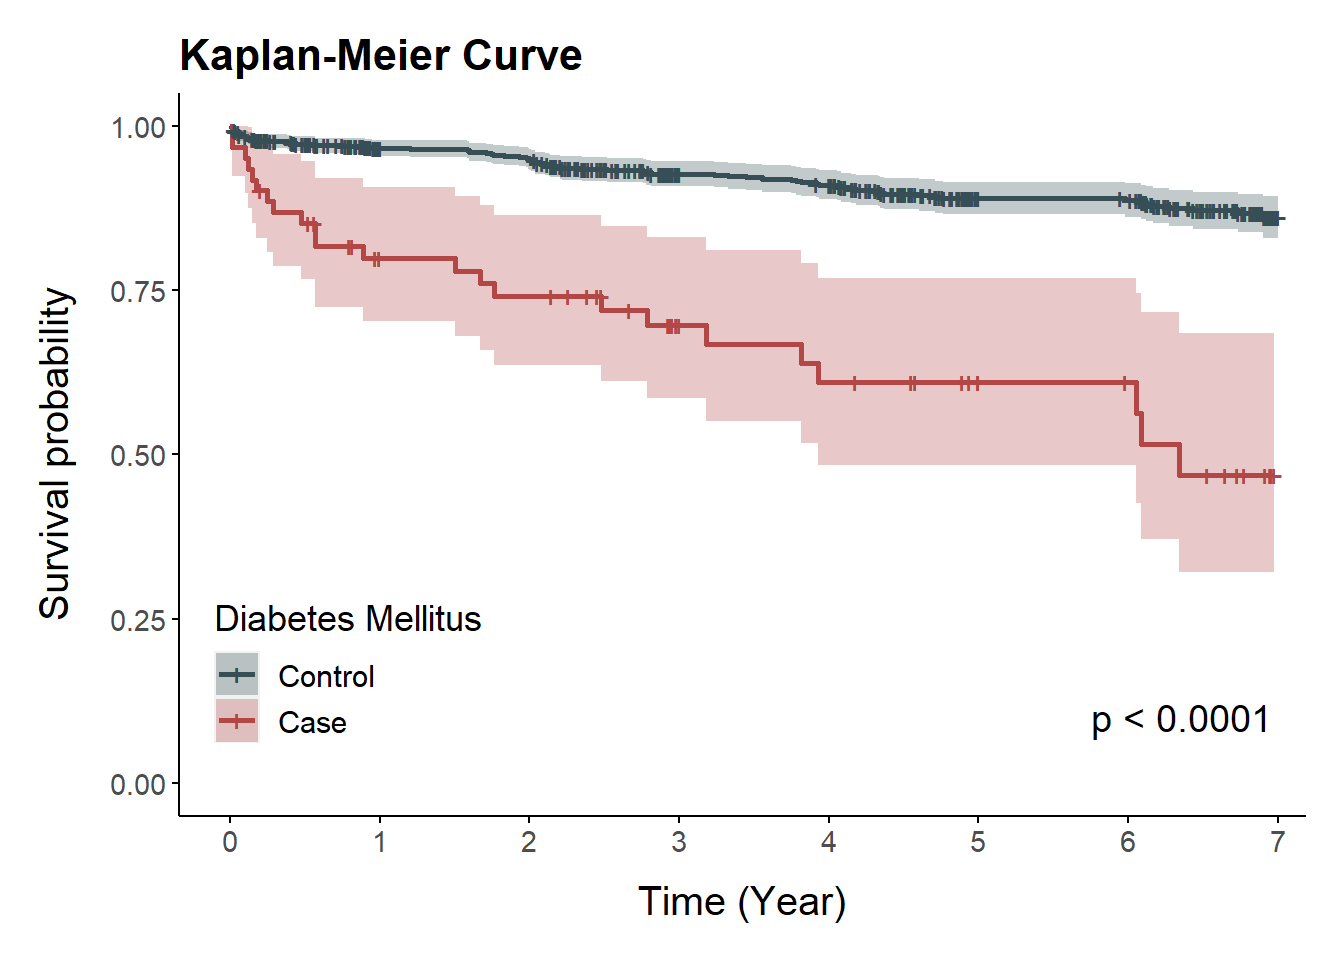
\includegraphics{bookdown_sample_files/figure-latex/unnamed-chunk-58-1.pdf}

\hypertarget{matching-version}{%
\subsection{Matching version}\label{matching-version}}

\begin{Shaded}
\begin{Highlighting}[]
\NormalTok{fit\_km }\OtherTok{\textless{}{-}} \FunctionTok{survfit}\NormalTok{(}\FunctionTok{Surv}\NormalTok{(DATEDIFF, HTN}\SpecialCharTok{==}\DecValTok{1}\NormalTok{)}\SpecialCharTok{\textasciitilde{}}\NormalTok{ DM, }\AttributeTok{data=}\NormalTok{dat\_mat, }\AttributeTok{weight =}\NormalTok{ weights)}
\FunctionTok{gg\_km}\NormalTok{(fit\_km)}
\end{Highlighting}
\end{Shaded}

\begin{verbatim}
## Scale for x is already present.
## Adding another scale for x, which will replace the existing scale.
\end{verbatim}

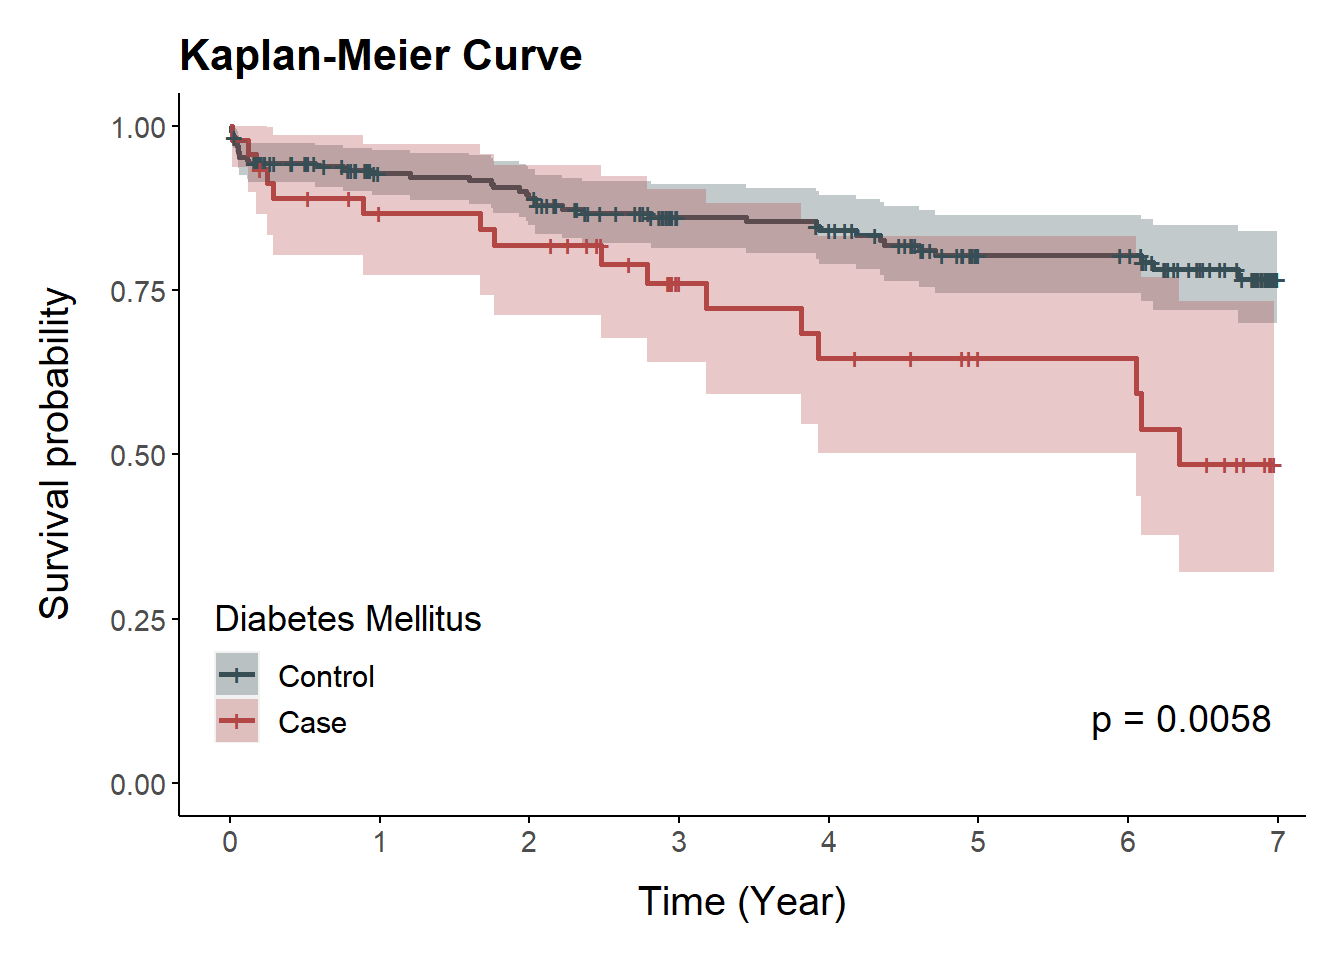
\includegraphics{bookdown_sample_files/figure-latex/unnamed-chunk-59-1.pdf}

\hypertarget{weighting-version}{%
\subsection{Weighting version}\label{weighting-version}}

\begin{Shaded}
\begin{Highlighting}[]
\NormalTok{fit\_km }\OtherTok{\textless{}{-}} \FunctionTok{survfit}\NormalTok{(}\FunctionTok{Surv}\NormalTok{(DATEDIFF, HTN}\SpecialCharTok{==}\DecValTok{1}\NormalTok{)}\SpecialCharTok{\textasciitilde{}}\NormalTok{ DM, }\AttributeTok{data=}\NormalTok{dat\_wt, }\AttributeTok{weight =}\NormalTok{ weights)}
\FunctionTok{gg\_km}\NormalTok{(fit\_km)}
\end{Highlighting}
\end{Shaded}

\begin{verbatim}
## Scale for x is already present.
## Adding another scale for x, which will replace the existing scale.
\end{verbatim}

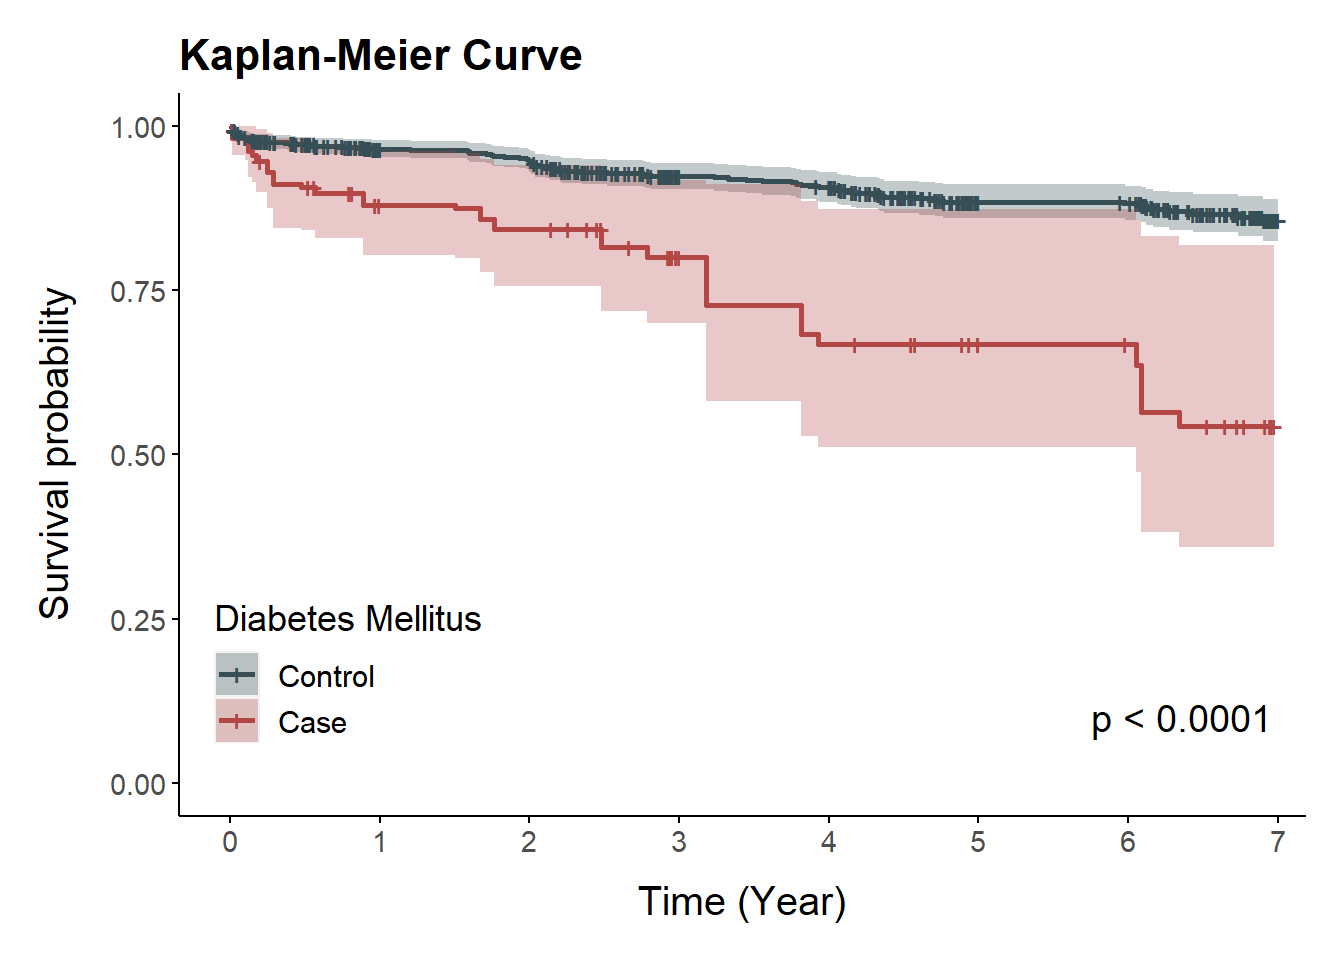
\includegraphics{bookdown_sample_files/figure-latex/unnamed-chunk-60-1.pdf}

\hypertarget{missing-data-version-2}{%
\section{Missing data version}\label{missing-data-version-2}}

\hypertarget{matching-version-1}{%
\subsection{Matching version}\label{matching-version-1}}

\begin{Shaded}
\begin{Highlighting}[]
\NormalTok{fit\_km }\OtherTok{\textless{}{-}} \FunctionTok{survfit}\NormalTok{(}\FunctionTok{Surv}\NormalTok{(DATEDIFF, HTN}\SpecialCharTok{==}\DecValTok{1}\NormalTok{)}\SpecialCharTok{\textasciitilde{}}\NormalTok{ DM, }\AttributeTok{data=}\NormalTok{dat\_mat\_list\_0}\FloatTok{.4}\NormalTok{[[}\DecValTok{1}\NormalTok{]])}
\FunctionTok{gg\_km}\NormalTok{(fit\_km)}
\end{Highlighting}
\end{Shaded}

\begin{verbatim}
## Scale for x is already present.
## Adding another scale for x, which will replace the existing scale.
\end{verbatim}

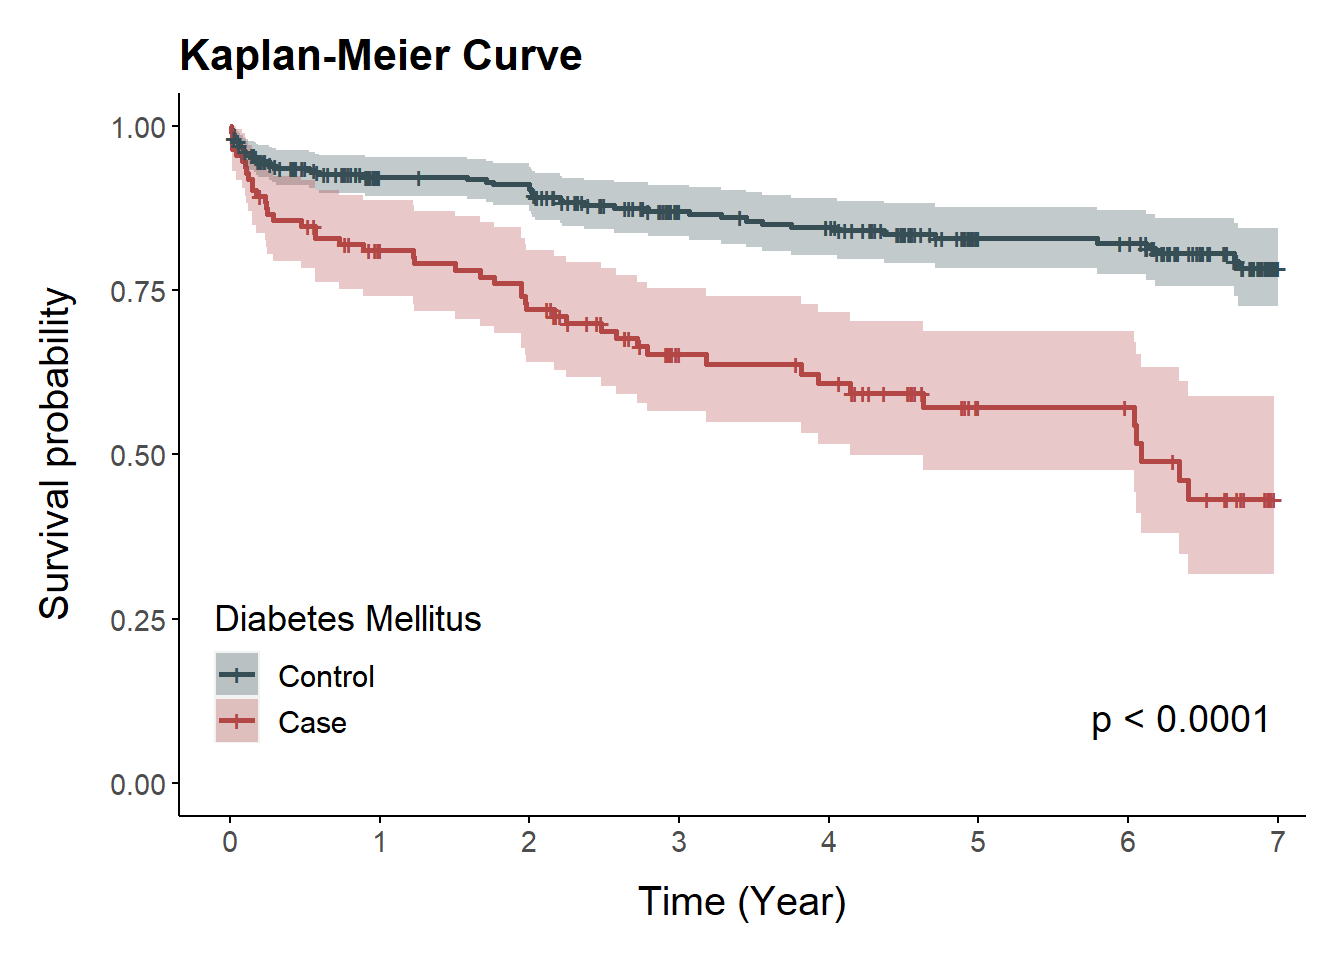
\includegraphics{bookdown_sample_files/figure-latex/unnamed-chunk-61-1.pdf}

\hypertarget{weighting-version-1}{%
\subsection{Weighting version}\label{weighting-version-1}}

\hypertarget{weighted-kaplan-meier-estimates}{%
\subsubsection{Weighted kaplan-meier estimates}\label{weighted-kaplan-meier-estimates}}

\begin{itemize}
\tightlist
\item
  Use \textbf{ipw.survival()} function in \textbf{RISCA} package to estimate adjusted survival curves by weighting the individual contributions by the inverse of the probability to be in the group (IPW).
\end{itemize}

\begin{Shaded}
\begin{Highlighting}[]
\NormalTok{surv\_res }\OtherTok{\textless{}{-}} \ControlFlowTok{function}\NormalTok{(data, time, status, group, formula)\{}
\NormalTok{  p.score }\OtherTok{\textless{}{-}} \FunctionTok{glm}\NormalTok{(}\AttributeTok{formula=}\NormalTok{formula, }\AttributeTok{data=}\NormalTok{data, }\AttributeTok{family=}\StringTok{"binomial"}\NormalTok{, }\AttributeTok{x=}\ConstantTok{TRUE}\NormalTok{, }\AttributeTok{y=}\ConstantTok{TRUE}\NormalTok{)}\SpecialCharTok{$}\NormalTok{fitted.values}
\NormalTok{  wt }\OtherTok{\textless{}{-}}\NormalTok{ (data[,group]}\SpecialCharTok{==}\StringTok{"1"}\NormalTok{)}\SpecialCharTok{/}\NormalTok{p.score }\SpecialCharTok{+}\NormalTok{ (data[,group]}\SpecialCharTok{==}\StringTok{"0"}\NormalTok{)}\SpecialCharTok{/}\NormalTok{(}\DecValTok{1}\SpecialCharTok{{-}}\NormalTok{p.score)}
\NormalTok{  pt }\OtherTok{\textless{}{-}} \FunctionTok{sum}\NormalTok{(data[,group]}\SpecialCharTok{==}\DecValTok{1}\NormalTok{)}\SpecialCharTok{/}\FunctionTok{nrow}\NormalTok{(data)}
\NormalTok{  sw }\OtherTok{\textless{}{-}}\NormalTok{ pt}\SpecialCharTok{*}\NormalTok{(data[,group]}\SpecialCharTok{==}\DecValTok{1}\NormalTok{) }\SpecialCharTok{/}\NormalTok{p.score }\SpecialCharTok{+}\NormalTok{ (}\DecValTok{1}\SpecialCharTok{{-}}\NormalTok{pt)}\SpecialCharTok{*}\NormalTok{(data[,group]}\SpecialCharTok{==}\DecValTok{0}\NormalTok{)}\SpecialCharTok{/}\NormalTok{(}\DecValTok{1}\SpecialCharTok{{-}}\NormalTok{p.score)}
\NormalTok{  res.akm }\OtherTok{\textless{}{-}} \FunctionTok{ipw.survival}\NormalTok{(}\AttributeTok{times=}\NormalTok{data[,time], }\AttributeTok{failures=}\NormalTok{data[,status], }\AttributeTok{variable=}\NormalTok{data[,group], }\AttributeTok{weights=}\NormalTok{sw)}
  \FunctionTok{return}\NormalTok{(res.akm)}
\NormalTok{\}}

\NormalTok{res.akm }\OtherTok{\textless{}{-}}\NormalTok{ dat\_imp\_list }\SpecialCharTok{\%\textgreater{}\%} \FunctionTok{lapply}\NormalTok{(}\ControlFlowTok{function}\NormalTok{(x) }\FunctionTok{surv\_res}\NormalTok{(x,}\StringTok{"DATEDIFF"}\NormalTok{,}\StringTok{"HTN"}\NormalTok{,}\StringTok{"DM"}\NormalTok{, formula.wt)}\SpecialCharTok{$}\NormalTok{table.surv)}
\NormalTok{risk }\OtherTok{\textless{}{-}} \FunctionTok{do.call}\NormalTok{(}\StringTok{"cbind"}\NormalTok{,res.akm }\SpecialCharTok{\%\textgreater{}\%} \FunctionTok{lapply}\NormalTok{(}\ControlFlowTok{function}\NormalTok{(x) x}\SpecialCharTok{$}\NormalTok{n.risk))}
\NormalTok{event }\OtherTok{\textless{}{-}} \FunctionTok{do.call}\NormalTok{(}\StringTok{"cbind"}\NormalTok{,res.akm }\SpecialCharTok{\%\textgreater{}\%} \FunctionTok{lapply}\NormalTok{(}\ControlFlowTok{function}\NormalTok{(x) x}\SpecialCharTok{$}\NormalTok{n.event))}
\NormalTok{surv }\OtherTok{\textless{}{-}} \FunctionTok{do.call}\NormalTok{(}\StringTok{"cbind"}\NormalTok{,res.akm }\SpecialCharTok{\%\textgreater{}\%} \FunctionTok{lapply}\NormalTok{(}\ControlFlowTok{function}\NormalTok{(x) x}\SpecialCharTok{$}\NormalTok{survival))}
\NormalTok{km\_res }\OtherTok{\textless{}{-}} \FunctionTok{data.frame}\NormalTok{(}\AttributeTok{time=}\NormalTok{res.akm[[}\DecValTok{1}\NormalTok{]]}\SpecialCharTok{$}\NormalTok{times, }\AttributeTok{strata=}\NormalTok{res.akm[[}\DecValTok{1}\NormalTok{]]}\SpecialCharTok{$}\NormalTok{variable,}
                     \AttributeTok{n.risk=}\FunctionTok{apply}\NormalTok{(risk,}\DecValTok{1}\NormalTok{,mean),}
                     \AttributeTok{n.event=}\FunctionTok{apply}\NormalTok{(event,}\DecValTok{1}\NormalTok{,mean),}
                     \AttributeTok{surv=}\FunctionTok{apply}\NormalTok{(surv,}\DecValTok{1}\NormalTok{,mean))}
\end{Highlighting}
\end{Shaded}

\begin{Shaded}
\begin{Highlighting}[]
\FunctionTok{head}\NormalTok{(km\_res)}
\end{Highlighting}
\end{Shaded}

\begin{verbatim}
##   time strata   n.risk  n.event      surv
## 1    0      0 2360.020 0.000000 1.0000000
## 2    2      0 2360.020 2.099422 0.9991104
## 3    5      0 2357.921 1.062941 0.9986600
## 4    6      0 2353.958 3.045573 0.9973680
## 5    7      0 2350.912 1.035237 0.9969288
## 6    9      0 2349.877 4.227905 0.9951351
\end{verbatim}

\hypertarget{kaplan-meier-curve-by-using-ipw}{%
\subsubsection{Kaplan-Meier curve by Using IPW}\label{kaplan-meier-curve-by-using-ipw}}

\begin{itemize}
\tightlist
\item
  Use \textbf{ggsurvplot\_df()} function in \textbf{survminer} package to plot survival curve from any data frame containing the summary of survival curves.
\end{itemize}

\begin{Shaded}
\begin{Highlighting}[]
\NormalTok{ggsurv\_plot }\OtherTok{\textless{}{-}} \FunctionTok{ggsurvplot\_df}\NormalTok{(km\_res,}
                             \AttributeTok{title =} \StringTok{"Kaplan{-}Meier Curve"}\NormalTok{,}
                             \AttributeTok{ggtheme =} \FunctionTok{theme}\NormalTok{(}\AttributeTok{axis.line =} \FunctionTok{element\_line}\NormalTok{(}\AttributeTok{color=}\StringTok{"black"}\NormalTok{),}
                                             \AttributeTok{panel.background =} \FunctionTok{element\_blank}\NormalTok{(),}
                                             \AttributeTok{plot.title =} \FunctionTok{element\_text}\NormalTok{(}\AttributeTok{hjust =} \DecValTok{0}\NormalTok{, }\AttributeTok{size=}\DecValTok{15}\NormalTok{, }\AttributeTok{face =} \StringTok{"bold"}\NormalTok{),}
                                             \AttributeTok{plot.margin =} \FunctionTok{unit}\NormalTok{(}\FunctionTok{c}\NormalTok{(}\DecValTok{5}\NormalTok{,}\DecValTok{3}\NormalTok{,}\DecValTok{5}\NormalTok{,}\DecValTok{5}\NormalTok{), }\StringTok{"mm"}\NormalTok{),}
                                             \AttributeTok{axis.title.y =} \FunctionTok{element\_text}\NormalTok{(}\AttributeTok{margin=}\FunctionTok{margin}\NormalTok{(}\AttributeTok{r=}\DecValTok{13}\NormalTok{)),}
                                             \AttributeTok{axis.title.x =} \FunctionTok{element\_text}\NormalTok{(}\AttributeTok{margin=}\FunctionTok{margin}\NormalTok{(}\AttributeTok{t=}\DecValTok{10}\NormalTok{)),}
                                             \AttributeTok{legend.background =}\FunctionTok{element\_blank}\NormalTok{(),}
                                             \AttributeTok{legend.text =} \FunctionTok{element\_text}\NormalTok{(}\AttributeTok{size =} \DecValTok{13}\NormalTok{, }\AttributeTok{color=}\StringTok{"black"}\NormalTok{),}
                                             \AttributeTok{legend.title =} \FunctionTok{element\_text}\NormalTok{( }\AttributeTok{size=}\FloatTok{13.5}\NormalTok{),}
                                             \AttributeTok{legend.spacing.x =} \FunctionTok{unit}\NormalTok{(}\FloatTok{0.5}\NormalTok{, }\StringTok{\textquotesingle{}cm\textquotesingle{}}\NormalTok{),}
                                             \AttributeTok{legend.spacing.y =} \FunctionTok{unit}\NormalTok{(}\FloatTok{0.3}\NormalTok{, }\StringTok{\textquotesingle{}cm\textquotesingle{}}\NormalTok{)),}
                             \AttributeTok{palette =} \FunctionTok{c}\NormalTok{(}\StringTok{"\#374E55FF"}\NormalTok{, }\StringTok{"\#B24745FF"}\NormalTok{),}
                             \AttributeTok{xlim =} \FunctionTok{c}\NormalTok{(}\DecValTok{0}\NormalTok{,}\DecValTok{2600}\NormalTok{),}
                             \AttributeTok{ylim =} \FunctionTok{c}\NormalTok{(}\FloatTok{0.5}\NormalTok{,}\DecValTok{1}\NormalTok{), }
                             \AttributeTok{size =} \FloatTok{1.2}\NormalTok{,}
                             \DocumentationTok{\#\#\# Format Axes (changes x,y axis label)}
                             \AttributeTok{xlab=}\StringTok{"Time (Years)"}\NormalTok{, }
                             \AttributeTok{font.x =} \FunctionTok{c}\NormalTok{(}\DecValTok{16}\NormalTok{), }
                             \AttributeTok{font.y =} \FunctionTok{c}\NormalTok{(}\DecValTok{16}\NormalTok{),}
                             \AttributeTok{font.tickslab =} \FunctionTok{c}\NormalTok{(}\DecValTok{13}\NormalTok{),}
                             \DocumentationTok{\#\#\# Format Legend}
                             \AttributeTok{legend.title =} \StringTok{"Diabetes Mellitus:  "}\NormalTok{,}
                             \AttributeTok{legend.labs =} \FunctionTok{c}\NormalTok{(}\StringTok{"Control"}\NormalTok{, }\StringTok{"Case"}\NormalTok{), }\CommentTok{\# Change the Strata Legend}
                             \AttributeTok{legend =} \FunctionTok{c}\NormalTok{(}\FloatTok{0.2}\NormalTok{,}\FloatTok{0.2}\NormalTok{) }
\NormalTok{                             ) }\SpecialCharTok{+} \FunctionTok{scale\_x\_continuous}\NormalTok{(}\AttributeTok{breaks =} \FunctionTok{c}\NormalTok{(}\DecValTok{0}\NormalTok{,}\FloatTok{730.5}\NormalTok{,}\DecValTok{1461}\NormalTok{,}\FloatTok{2191.5}\NormalTok{,}\DecValTok{2922}\NormalTok{,}\FloatTok{3652.5}\NormalTok{), }\AttributeTok{labels =} \FunctionTok{c}\NormalTok{(}\DecValTok{0}\NormalTok{,}\DecValTok{2}\NormalTok{,}\DecValTok{4}\NormalTok{,}\DecValTok{6}\NormalTok{,}\DecValTok{8}\NormalTok{,}\DecValTok{10}\NormalTok{))}
\end{Highlighting}
\end{Shaded}

\begin{verbatim}
## Scale for x is already present.
## Adding another scale for x, which will replace the existing scale.
\end{verbatim}

\begin{Shaded}
\begin{Highlighting}[]
\NormalTok{ggsurv\_plot}
\end{Highlighting}
\end{Shaded}

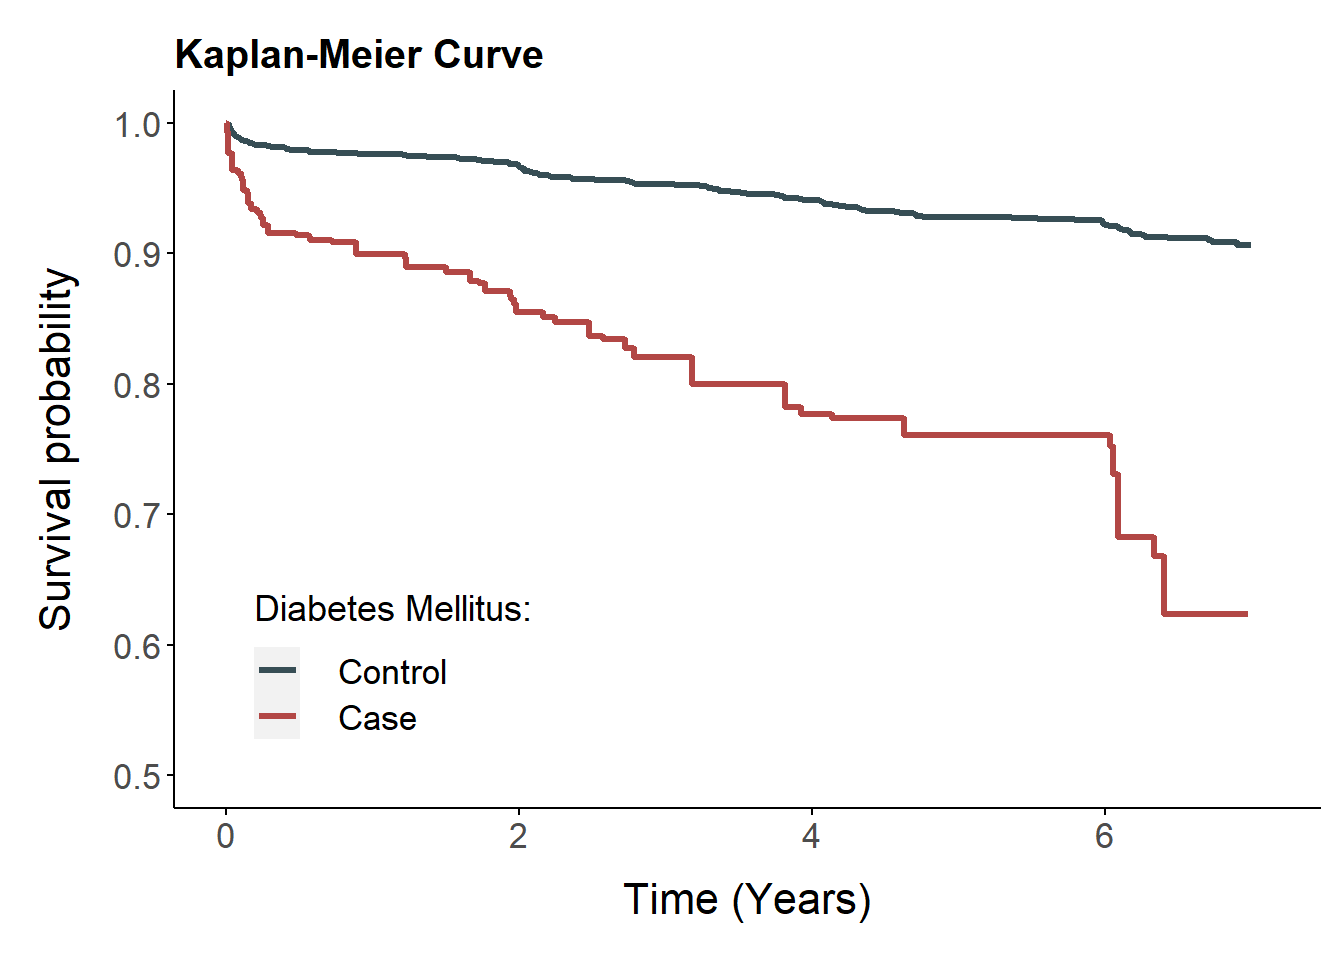
\includegraphics{bookdown_sample_files/figure-latex/unnamed-chunk-64-1.pdf}

\hypertarget{logistic-regression}{%
\chapter{Logistic regression}\label{logistic-regression}}

\begin{longtable}[]{@{}l@{}}
\toprule()
\endhead
Using data \textbf{final\_com, dat\_mat, dat\_wt} (complete data version) \\
Using list \textbf{dat\_mat\_list, dat\_imp\_list} (missing data version) \\
Outcome variable : \textbf{HTN} \\
Follow-up period : \textbf{DATEDIFF} \\
Exposure variable : \textbf{DM} \\
Covariates : \textbf{Age, Sex, SES, Region, BMI, CCI, Comorbidities(Dyslipidemia, Ischemic heart disease)} \\
\bottomrule()
\end{longtable}

\begin{Shaded}
\begin{Highlighting}[]
\DocumentationTok{\#\# load library}
\FunctionTok{library}\NormalTok{(survival)}
\FunctionTok{library}\NormalTok{(survminer)}
\FunctionTok{library}\NormalTok{(ggsci)}
\FunctionTok{library}\NormalTok{(RISCA) }\CommentTok{\# 서버에서는 library(IPWsurvival) 사용}
\end{Highlighting}
\end{Shaded}

\begin{Shaded}
\begin{Highlighting}[]
\DocumentationTok{\#\# load data}
\NormalTok{final\_com }\OtherTok{\textless{}{-}} \FunctionTok{read.csv}\NormalTok{(}\StringTok{\textquotesingle{}Data/final\_com.csv\textquotesingle{}}\NormalTok{, }\AttributeTok{header=}\NormalTok{T)}
\FunctionTok{load}\NormalTok{(}\StringTok{"Data/dat\_mat.RData"}\NormalTok{)}
\FunctionTok{load}\NormalTok{(}\StringTok{"Data/dat\_wt.RData"}\NormalTok{)}
\FunctionTok{load}\NormalTok{(}\StringTok{"Data/dat\_mat\_list\_0.4.RData"}\NormalTok{)}
\FunctionTok{load}\NormalTok{(}\StringTok{"Data/dat\_imp\_list.RData"}\NormalTok{)}
\end{Highlighting}
\end{Shaded}

\begin{Shaded}
\begin{Highlighting}[]
\DocumentationTok{\#\# Formula}
\NormalTok{formula.wt }\OtherTok{\textless{}{-}} \FunctionTok{formula}\NormalTok{(DM }\SpecialCharTok{\textasciitilde{}}\NormalTok{ AGE }\SpecialCharTok{+}\NormalTok{ SEX }\SpecialCharTok{+}\NormalTok{ SES }\SpecialCharTok{+}\NormalTok{ REGION }\SpecialCharTok{+}\NormalTok{ BMI }\SpecialCharTok{+}\NormalTok{ CCI }\SpecialCharTok{+}\NormalTok{ DYS }\SpecialCharTok{+}\NormalTok{ IHD)}
\end{Highlighting}
\end{Shaded}

\begin{center}\rule{0.5\linewidth}{0.5pt}\end{center}

  \bibliography{book.bib,packages.bib}

\end{document}
